% !TeX encoding = UTF-8
% !TeX program = xelatex
% !TeX spellcheck = en_US

\documentclass[degree=master]{thuthesis}
  % 学位 degree:
  %   doctor | master | bachelor | postdoc
  % 学位类型 degree-type:
  %   academic(默认)| professional
  % 语言 language
  %   chinese(默认)| english
  % 字体库 fontset
  %   windows | mac | fandol | ubuntu
  % 建议终版使用 Windows 平台的字体编译


% 论文基本配置,加载宏包等全局配置
% !TeX root = ./thuthesis-example.tex

% 论文基本信息配置

\thusetup{
  %******************************
  % 注意:
  %   1. 配置里面不要出现空行
  %   2. 不需要的配置信息可以删除
  %   3. 建议先阅读文档中所有关于选项的说明
  %******************************
  %
  % 输出格式
  %   选择打印版(print)或用于提交的电子版(electronic),前者会插入空白页以便直接双面打印
  %
  output = print,
  %
  % 标题
  %   可使用“\\”命令手动控制换行
  %
  title  = {基于扩散模型的图像去噪算法},
  title* = {An Image Restoration Algorithm Based  Diffusion Model},
  %
  % 学科门类
  %   1. 学术型
  %      - 中文
  %        需注明所属的学科门类,例如:
  %        哲学、经济学、法学、教育学、文学、历史学、理学、工学、农学、医学、
  %        军事学、管理学、艺术学
  %      - 英文
  %        博士:Doctor of Philosophy
  %        硕士:
  %          哲学、文学、历史学、法学、教育学、艺术学门类,公共管理学科
  %          填写“Master of Arts“,其它填写“Master of Science”
  %   2. 专业型
  %      直接填写专业学位的名称,例如:
  %      教育博士、工程硕士等
  %      Doctor of Education, Master of Engineering
  %   3. 本科生不需要填写
  %
  degree-category  = {数学系学士},
  degree-category* = {Bachelor of Science},
  %
  % 培养单位
  %   填写所属院系的全名
  %
  department = {数学科学系},
  %
  % 学科
  %   1. 研究生学术型学位,获得一级学科授权的学科填写一级学科名称,其他填写二级学科名称
  %   2. 本科生填写专业名称,第二学位论文需标注“(第二学位)”
  %
  discipline  = {数学与应用数学},
  discipline* = {Department of Mathematical Science},
  %
  % 专业领域
  %   1. 设置专业领域的专业学位类别,填写相应专业领域名称
  %   2. 2019 级及之前工程硕士学位论文,在 `engineering-field` 填写相应工程领域名称
  %   3. 其他专业学位类别的学位论文无需此信息
  %
  % professional-field  = {计算机技术},
  % professional-field* = {Computer Technology},
  %
  % 姓名
  %
  author  = {郭骏宇},
  author* = {Guo Junyu},
  %
  % 指导教师
  %   中文姓名和职称之间以英文逗号“,”分开,下同
  %
  supervisor  = {包承龙, 助理教授},
  supervisor* = {Professor Bao Chenglong},
  %
  % 副指导教师
  %
  % associate-supervisor  = {陈文光, 教授},
  % associate-supervisor* = {Professor Chen Wenguang},
  %
  % 联合指导教师
  %
  % co-supervisor  = {某某某, 教授},
  % co-supervisor* = {Professor Mou Moumou},
  %
  % 日期
  %   使用 ISO 格式;默认为当前时间
  %
  % date = {2019-07-07},
  %
  % 是否在中文封面后的空白页生成书脊(默认 false)
  %
  include-spine = false,
  %
  % 密级和年限
  %   秘密, 机密, 绝密
  %
  % secret-level = {秘密},
  % secret-year  = {10},
  %
  % 博士后专有部分
  %
  % clc                = {分类号},
  % udc                = {UDC},
  % id                 = {编号},
  % discipline-level-1 = {计算机科学与技术},  % 流动站(一级学科)名称
  % discipline-level-2 = {系统结构},          % 专业(二级学科)名称
  % start-date         = {2011-07-01},        % 研究工作起始时间
}

% 载入所需的宏包

% 定理类环境宏包
\usepackage{amsthm}
% 也可以使用 ntheorem
% \usepackage[amsmath,thmmarks,hyperref]{ntheorem}

\thusetup{
  %
  % 数学字体
  % math-style = GB,  % GB | ISO | TeX
  math-font  = xits,  % stix | xits | libertinus
}

% 可以使用 nomencl 生成符号和缩略语说明
% \usepackage{nomencl}
% \makenomenclature

% 表格加脚注
\usepackage{threeparttable}

% 表格中支持跨行
\usepackage{multirow}

% 固定宽度的表格。
% \usepackage{tabularx}

% 跨页表格
\usepackage{longtable}

% 算法
\usepackage{algorithm}
\usepackage{algorithmic}

% 量和单位
\usepackage{siunitx}

% 参考文献使用 BibTeX + natbib 宏包
% 顺序编码制
\usepackage[sort]{natbib}
\bibliographystyle{thuthesis-numeric}

% 著者-出版年制
% \usepackage{natbib}
% \bibliographystyle{thuthesis-author-year}

% 本科生参考文献的著录格式
% \usepackage[sort]{natbib}
% \bibliographystyle{thuthesis-bachelor}

% 参考文献使用 BibLaTeX 宏包
% \usepackage[style=thuthesis-numeric]{biblatex}
% \usepackage[style=thuthesis-author-year]{biblatex}
% \usepackage[style=apa]{biblatex}
% \usepackage[style=mla-new]{biblatex}
% 声明 BibLaTeX 的数据库
% \addbibresource{ref/refs.bib}

% 定义所有的图片文件在 figures 子目录下
\graphicspath{{figures/}}

% 数学命令
\makeatletter
\newcommand\dif{%  % 微分符号
  \mathop{}\!%
  \ifthu@math@style@TeX
    d%
  \else
    \mathrm{d}%
  \fi
}
\makeatother

% hyperref 宏包在最后调用
\usepackage{hyperref}



\begin{document}

% 封面
\maketitle

% 学位论文指导小组、公开评阅人和答辩委员会名单
% 本科生不需要
% % !TeX root = ../thuthesis-example.tex

\begin{committee}[name={学位论文指导小组、公开评阅人和答辩委员会名单}]

  \newcolumntype{C}[1]{@{}>{\centering\arraybackslash}p{#1}}

  \section*{指导小组名单}

  \begin{center}
    \begin{tabular}{C{3cm}C{3cm}C{9cm}@{}}
      李XX & 教授     & 清华大学 \\
      王XX & 副教授   & 清华大学 \\
      张XX & 助理教授 & 清华大学 \\
    \end{tabular}
  \end{center}


  \section*{公开评阅人名单}

  \begin{center}
    \begin{tabular}{C{3cm}C{3cm}C{9cm}@{}}
      刘XX & 教授   & 清华大学                    \\
      陈XX & 副教授 & XXXX大学                    \\
      杨XX & 研究员 & 中国XXXX科学院XXXXXXX研究所 \\
    \end{tabular}
  \end{center}


  \section*{答辩委员会名单}

  \begin{center}
    \begin{tabular}{C{2.75cm}C{2.98cm}C{4.63cm}C{4.63cm}@{}}
      主席 & 赵XX                  & 教授                    & 清华大学       \\
      委员 & 刘XX                  & 教授                    & 清华大学       \\
          & \multirow{2}{*}{杨XX} & \multirow{2}{*}{研究员} & 中国XXXX科学院 \\
          &                       &                         & XXXXXXX研究所  \\
          & 黄XX                  & 教授                    & XXXX大学       \\
          & 周XX                  & 副教授                  & XXXX大学       \\
      秘书 & 吴XX                  & 助理研究员              & 清华大学       \\
    \end{tabular}
  \end{center}

\end{committee}



% 也可以导入 Word 版转的 PDF 文件
% \begin{committee}[file=figures/committee.pdf]
% \end{committee}



% 使用授权的说明
\copyrightpage
% 将签字扫描后授权文件 scan-copyright.pdf 替换原始页面
% \copyrightpage[file=scan-copyright.pdf]

\frontmatter
% !TeX root = ../thuthesis-example.tex

% 中英文摘要和关键字

\begin{abstract}
在当今数字图像处理与计算机视觉领域,图像去噪及图像生成是核心且至关重要的问题。近年来,机器学习方法的崛起使得高质量图像的生成成为研究焦点,其中扩散模型因其出色的生成效果而受到广泛关注。深度扩散模型,由正向扩散与逆向采样两部分构成,通过训练及采样过程,逐渐逼近目标图像的分布。

然而,在图像条件生成领域,深度学习驱动的扩散模型面临着训练难度高、表达能力有限及泛化能力不足的挑战。首先,现有模型对输入图像的噪声较为敏感,缺乏足够的鲁棒性。其次,针对特定数据集训练的扩散模型成本高昂,如何有效利用预训练集辅助条件生成成为一大难题。最后,在模型泛化方面,如何设计适用于不同图像条件生成任务(如图像修复、去模糊、超分辨率等)的高效算法,成为当前研究的热点。

针对上述问题,本文提出了一种高效的图像条件生成算法,其创新点主要体现在以下三个方面:

首先,针对深度学习模型对噪声输入不鲁棒的问题,本文提出了一种基于扩散模型的图像去噪算法,该算法通过对后验分布似然函数的逼近,实现了对输入噪声的稳定去噪。相较于传统模型,该算法不仅具有更好的表达能力,而且函数族严格包含已有模型的函数族。

其次,针对DDPM采样方法训练开销大的问题,本文利用DDIM模型中的采样方法进行分段采样,有效减少了迭代次数,从而降低了生成图片数量较大时的训练成本,使得图像修复算法得以高效实现。

最后,针对条件生成算法中采样速度慢及学习率调整复杂的问题,本文提出了一种无模型依赖的学习率设置算法。该算法经过实验验证,适用于LSUN、Imagenet及FFHQ等数据集,显著提高了条件生成算法的稳定性。

综上所述,本文提出的算法在图像条件生成领域具有显著的创新性和实用性,为解决当前存在的问题提供了新的思路和方法。
  \thusetup{
    keywords = { 图像修复 ,扩散模型, 神经网络, 后验估计, 分层模型},
  }
\end{abstract}

\begin{abstract*}
In the current field of digital image processing and computer vision, image denoising and generation have always been crucial issues. In recent years, the rise of machine learning methods has made the generation of high-quality images a research focus, with diffusion models receiving widespread attention due to their excellent generation effects. Deep diffusion models, consisting of forward diffusion and reverse sampling processes, gradually approximate the distribution of target images through training and sampling.

However, in the realm of conditional image generation, deep learning-driven diffusion models face challenges in terms of training difficulty, limited expressive power, and insufficient generalization ability. Firstly, existing models are sensitive to noise in input images and lack sufficient robustness. Secondly, the cost of training diffusion models for specific datasets is high, and how to effectively utilize pre-trained sets to assist in conditional generation has become a major challenge. Finally, in terms of model generalization, designing efficient algorithms suitable for different conditional image generation tasks such as image restoration, deblurring, and super-resolution has become a hotspot in current research.

In response to the above issues, this paper proposes an efficient algorithm for conditional image generation. The main innovations are reflected in the following three aspects:

Firstly, addressing the issue of deep learning models' lack of robustness to noisy inputs, this paper proposes an image denoising algorithm based on diffusion models. By approximating the likelihood function of the posterior distribution, the algorithm achieves stable denoising of input noise. Compared to traditional models, it not only exhibits better expressive power but also strictly contains the function families of existing models.

Secondly, to address the high training cost associated with the DDPM sampling method, this paper utilizes the sampling method from the DDIM model to perform segmented sampling, effectively reducing the number of iterations. This approach lowers the training cost when generating a large number of images, enabling efficient implementation of image restoration algorithms.

Finally, addressing the issues of slow sampling speed and the complexity of manually adjusting learning rates in conditional generation algorithms, this paper proposes a model-free learning rate setting algorithm. Experimental verification has shown that this algorithm is suitable for datasets such as LSUN, Imagenet, and FFHQ, significantly improving the stability of conditional generation algorithms.

In summary, the algorithm proposed in this paper exhibits significant innovation and practicality in the field of conditional image generation, providing new ideas and methods for addressing existing problems.

  % Use comma as separator when inputting
  \thusetup{
    keywords* = {Image Restoration, Diffusion Model, Neural Network, Posterior Estimation, Stratified Model},
  }
\end{abstract*}


% 目录
\tableofcontents

% 插图和附表清单
% 本科生的插图索引和表格索引需要移至正文之后、参考文献前
% \listoffiguresandtables  % 插图和附表清单(仅限研究生)
\listoffigures           % 插图清单
\listoftables            % 附表清单

% 符号对照表
% !TeX root = ../thuthesis-example.tex

\begin{denotation}[3cm]
  \item[$q_{\phi}(z|x)$] 表示VAE模型中的编码器,其中$\phi$为编码器的参数
  \item [$p_{\theta}(x|z)$] 表示VAE模型中的解码器,其中$\theta$代表解码器的参数
  \item [ELBO] Evident Lower Bound, 在VAE模型中使用极大似然估计进行参数拟合,在此兼顾计算效率不直接对似然函数进行极大化而对似然函数的下界进行优化,将该目标函数称为ELBO
  \item [$q(z_t)$]表示在扩散模型中正向传播过程中随机变量的密度函数
  \item [$q(z_t\mid z_{t-1})$] 表示在扩散模型中正向传播过程中随机变量的条件分布的密度函数
  \item [$s_{\theta}(x,t)$] Score function, 在Diffusion Model 中用来计算逆向SDE的关键函数
  \item [$p({x}_t\mid y)$] 条件似然函数,用于生成条件生成中需要拟合的新的Score function
  \item [$\nabla_{{x}_t}\log\left(p({x}_t\mid y)\right)$] 条件生成问题下的Score function
  \item [Score matching] 通过参数拟合学习得到正确的Score function的过程

  \item [Diffusion SDE] 扩散随机微分方程(diffusion stochastic differential equation)

  \item [KL 散度] 库尔贝克-莱布勒散度(Kullback-Leibler divergence)
  \item [$p(\cdot)$] 概率密度函数
  \item [$\boldsymbol{x}$] 向量随机变量
  \item [$p(\cdot;\theta)$] 由 $\theta$ 参数化的概率分布 $p(\cdot)$ 的概率密度函数
  \item [$\mathbb{P}(\cdot)$] 概率值
  \item [$\alpha_t$] 扩散模型前向过程中均值的系数
  \item [$\sigma_t$] 扩散模型前向过程中的标准差
  \item [$\mathbb{R}$] 实数空间
  \item [$\operatorname{Id}$] 恒等映射(identity mapping)

\item [$\operatorname{det}(\cdot)$] 矩阵的行列式
\item[$\circ$] 矩阵的复合
\item[$\|\cdot \|_1$] 矩阵/向量的1-范数

\item[$\|\cdot \|_2$] 矩阵/向量的1-范数

\item[$f^{-1}$] 函数$f$的逆函数

\item[ $\epsilon_{\theta}$] 由参数 $\theta$ 定义的噪声预测模型(


  
  
  
  
  
\end{denotation}



% 也可以使用 nomencl 宏包,需要在导言区
% \usepackage{nomencl}
% \makenomenclature

% 在这里输出符号说明
% \printnomenclature[3cm]

% 在正文中的任意为都可以标题
% \nomenclature{PI}{聚酰亚胺}
% \nomenclature{MPI}{聚酰亚胺模型化合物,N-苯基邻苯酰亚胺}
% \nomenclature{PBI}{聚苯并咪唑}
% \nomenclature{MPBI}{聚苯并咪唑模型化合物,N-苯基苯并咪唑}
% \nomenclature{PY}{聚吡咙}
% \nomenclature{PMDA-BDA}{均苯四酸二酐与联苯四胺合成的聚吡咙薄膜}
% \nomenclature{MPY}{聚吡咙模型化合物}
% \nomenclature{As-PPT}{聚苯基不对称三嗪}
% \nomenclature{MAsPPT}{聚苯基不对称三嗪单模型化合物,3,5,6-三苯基-1,2,4-三嗪}
% \nomenclature{DMAsPPT}{聚苯基不对称三嗪双模型化合物(水解实验模型化合物)}
% \nomenclature{S-PPT}{聚苯基对称三嗪}
% \nomenclature{MSPPT}{聚苯基对称三嗪模型化合物,2,4,6-三苯基-1,3,5-三嗪}
% \nomenclature{PPQ}{聚苯基喹噁啉}
% \nomenclature{MPPQ}{聚苯基喹噁啉模型化合物,3,4-二苯基苯并二嗪}
% \nomenclature{HMPI}{聚酰亚胺模型化合物的质子化产物}
% \nomenclature{HMPY}{聚吡咙模型化合物的质子化产物}
% \nomenclature{HMPBI}{聚苯并咪唑模型化合物的质子化产物}
% \nomenclature{HMAsPPT}{聚苯基不对称三嗪模型化合物的质子化产物}
% \nomenclature{HMSPPT}{聚苯基对称三嗪模型化合物的质子化产物}
% \nomenclature{HMPPQ}{聚苯基喹噁啉模型化合物的质子化产物}
% \nomenclature{PDT}{热分解温度}
% \nomenclature{HPLC}{高效液相色谱(High Performance Liquid Chromatography)}
% \nomenclature{HPCE}{高效毛细管电泳色谱(High Performance Capillary lectrophoresis)}
% \nomenclature{LC-MS}{液相色谱-质谱联用(Liquid chromatography-Mass Spectrum)}
% \nomenclature{TIC}{总离子浓度(Total Ion Content)}
% \nomenclature{\textit{ab initio}}{基于第一原理的量子化学计算方法,常称从头算法}
% \nomenclature{DFT}{密度泛函理论(Density Functional Theory)}
% \nomenclature{$E_a$}{化学反应的活化能(Activation Energy)}
% \nomenclature{ZPE}{零点振动能(Zero Vibration Energy)}
% \nomenclature{PES}{势能面(Potential Energy Surface)}
% \nomenclature{TS}{过渡态(Transition State)}
% \nomenclature{TST}{过渡态理论(Transition State Theory)}
% \nomenclature{$\increment G^\neq$}{活化自由能(Activation Free Energy)}
% \nomenclature{$\kappa$}{传输系数(Transmission Coefficient)}
% \nomenclature{IRC}{内禀反应坐标(Intrinsic Reaction Coordinates)}
% \nomenclature{$\nu_i$}{虚频(Imaginary Frequency)}
% \nomenclature{ONIOM}{分层算法(Our own N-layered Integrated molecular Orbital and molecular Mechanics)}
% \nomenclature{SCF}{自洽场(Self-Consistent Field)}
% \nomenclature{SCRF}{自洽反应场(Self-Consistent Reaction Field)}



% 正文部分
\mainmatter


\chapter{引言}
\section{问题介绍}

在当今数字图像处理和计算机视觉领域,图像去噪一直是一个至关重要的问题。在实际应用中,由于各种因素,例如传感器噪声、压缩、低光条件等,图像中常常存在噪声,这会影响到图像的质量和后续处理任务的准确性。如何从现实中实际获取带噪图像中还原得到原先清晰度更高的原始图像具有重大的应用价值和前景。
因此,开发高效准确的图像去噪算法对于提升图像质量以及下游任务的性能具有重要意义。
\subsection*{图像去噪的挑战}
传统的图像去噪方法通常基于滤波器和统计学方法,它们可以在某些场景下取得不错的效果。然而,在面对复杂的噪声分布或者噪声与信号之间相互重叠的情况下,传统方法的性能往往受到限制。特别是对于低信噪比(SNR)的图像,传统方法可能会产生过度平滑或者细节损失的问题。      

若利用传统统计学习方法来进行图像处理,则通常将二维图像当作一维向量进行处理。图像作为一类特殊的数据类型其分布通常可以被看作在高维向量空间中的一个低维流形的嵌入,即在图像中通常有较多常见特征反复出现,使得其有相比于一般向量空间中数据分布的特殊性质,若对其向量化则会失去一部分图像数据分布独有的特征。
\subsection*{引入深度学习}
近年来,随着深度学习技术的发展,基于深度学习的图像去噪方法逐渐受到关注。其中,Variational Autoencoder(VAE)和Diffusion Model (DM)等深度生成模型因其能够学习到图像的复杂概率分布而备受瞩目。这些模型不仅能够准确地去除噪声,还可以保留图像的细节和结构,从而在实际应用中取得更好的效果。
\section{选题背景及意义}

\subsection*{选题背景}
随着数字图像在日常生活和工业应用中的普及,图像质量的要求越来越高。然而,在现实世界中,图像往往会受到各种形式的干扰和噪声,例如传感器噪声、压缩引起的伪像、低光条件下的图像模糊等。这些噪声不仅降低了图像的质量,还可能影响后续的图像分析和处理任务的准确性和可靠性。\par 
传统的图像去噪方法通常基于数学模型和信号处理技术,例如中值滤波、高斯滤波等。然而,这些方法往往只能处理特定类型的噪声,对于复杂的噪声分布或者噪声与信号之间的相互干扰,传统方法的效果可能不尽如人意,具有较大的局限性。
\subsection*{选题意义}
提升图像质量: 有效的图像去噪算法可以帮助提升图像的质量,使其更加清晰和真实,提高观感体验。\par 
改善后续处理任务的效果: 在许多图像处理和分析任务中,图像质量对结果的影响至关重要。去噪后的图像更容易进行特征提取、对象检测、图像识别等后续处理任务,从而提高了这些任务的准确性和鲁棒性。\par 
推动深度学习在图像处理领域的应用: 结合VAE和Diffusion Model等深度生成模型进行图像去噪不仅可以提高去噪效果,还可以推动深度学习技术在图像处理领域的应用。通过将深度学习引入图像去噪领域,可以充分挖掘图像数据的潜在信息,实现更加智能和高效的图像处理算法。\par 
实践应用的需求: 在实际应用中,如医学影像、卫星图像、安防监控等领域,图像质量对于决策和诊断的重要性不言而喻。因此,开发高效准确的图像去噪算法对于满足实践应用的需求具有重要意义。\par 
综上所述,研究图像去噪算法不仅有助于提升图像质量和后续处理任务的效果,还有助于推动深度学习技术在图像处理领域的应用,满足实际应用的需求,具有重要的理论和实践意义。
\subsection*{本研究的目的}
本研究旨在探索如何结合VAE和Diffusion Model这两种先进的深度生成模型来解决图像去噪问题。通过结合VAE的自编码器结构和Diffusion Model的概率建模能力,我们希望实现对于不同类型噪声的鲁棒去除,并保持图像的真实性和细节。本研究的结果不仅可以提升图像去噪的效果,还可能对于其他相关领域,如图像增强和图像重建等,产生积极的影响。通过对图像去噪问题的深入研究,我们有望为实际应用提供更加鲁棒和可靠的解决方案,推动计算机视觉技术在实践中的进一步发展。
\section{论文结构安排}
首先,在第二章进行图像修复相关文献回顾,包括传统非条件生成下的VAE模型到扩散模型,再到当今最高效的stable diffusion的原理,回顾了如何用如上无监督学习下的深度学习算法来高效学习到原数据集的总体分布。     

在第三章引入本文主要讨论主题:即图像修复的下游任务,阐述本文主要的研究目的与具体研究问题阐释。      

在第四章中,主要对实验细节和参数设定进行讨论,展示了本文在工程实现图像去噪任务中的贡献。 并且对条件生成下在不同算法下的生成图像质量进行分析比较,从而论证了本文所提出算法的优越性。     

最后,在第五章中,对图像修复任务的未来进行展望,总结了在未来可以有的提升方向。 

% \section{引言的写法}

% 一篇学位论文的引言大致包含如下几个部分:
% 1、问题的提出;
% 2、选题背 景及意义;
% 3、文献综述;
% 4、研究方法;
% 5、论文结构安排。
% \begin{itemize}
%   \item 问题的提出:要清晰地阐述所要研究的问题“是什么”。
%     \footnote{选题时切记要有“问题意识”,不要选不是问题的问题来研究。}
%   \item 选题背景及意义:论述清楚为什么选择这个题目来研究,即阐述该研究对学科发展的贡献、对国计民生的理论与现实意义等。
%   \item 文献综述:对本研究主题范围内的文献进行详尽的综合述评,“述”的同时一定要有“评”,指出现有研究状态,仍存在哪些尚待解决的问题,讲出自己的研究有哪些探索性内容。
%   \item 研究方法:讲清论文所使用的学术研究方法。
%   \item 论文结构安排:介绍本论文的写作结构安排。
% \end{itemize}

\chapter{文献回顾}
\section{变分编码器(VAE Model)}
变分编码器(Variational Auto Encoder Model)是一个有效学习未知高维数据分布的生成式模型,广泛应用于图像,音频,视频等数据用用于生成相似分布的数据。在诸多Bayes模型中,通常需要构造隐式变量(Latent Variable)去用来刻画目标分布,然而通常对于隐式变量的后验分布是没有任何额外信息的,同时在许多模型下也不存在解析表达式。\par 
首先明确VAE模型的适用问题范围,VAE模型主要用来处理i.i.d型数据点样本,利用变分推断等方法获得对该连续分布数据的逼近。
在VAE模型中,引入了编码器(Encoder)用来逼近隐式变量的后验分布(基于现有样本),利用变分推断、极大似然估计等技术来训练解码器(Decoder),从而利用隐式变量生成对目标样本分布的逼近。以下为变分编码器构成的图例,在图\ref{VAE model fig}中,首先中,首先将原始数据点作为输入,利用编码器可生成隐式变量。通过在隐式变量空间中重新采样,可以重新通过解码器映射到样本空间中,生成对原样本分布的逼近。
\begin{figure}[H]
    \centering
    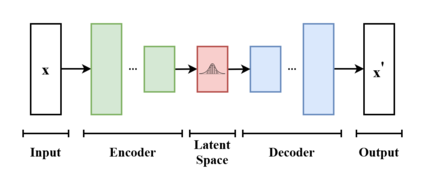
\includegraphics[scale = 0.7]{ThuThesis_ Tsinghua University Thesis LaTeX Template/Picture/VAE.png}
    \caption{VAE 模型构成}
    \label{VAE model fig}
\end{figure}
以上为VAE模型的总体架构说明,接下来的部分将对VAE模型的数学原理进行说明。VAE模型同传统贝叶斯模型一样,同样采用极大似然估计的方法(MLE)对参数进行估计。不同点在于不直接对似然函数进行优化,采用变分推断的方法对对数似然函数的相反数下界进行极小化。该方法避免了不存在解析解的困境,易于数值计算提升优化效率。接下来定义相关符号,在VAE模型中,解码器为$p_{\theta}(x|z)$,在给定了隐式变量$z$的情况下通过以$\theta$为参数化的模型定义了一个条件概率分布。编码器$q_{\phi}(z|x)$,用来逼近真实的后验分布$p_{\theta}(z|x)$。与传统的Bayes模型不同的地方在于,编码器和解码器不直接定义从样本空间和隐式空间之间的具体映射,而是从一个空间的样本定义在另一个空间内样本的分布,再通过采样的方式获得。假设给定样本点为$\{x^1,\cdots,x^{N}\}$,在MLE的原则下,我们的目标是极大化$\mathbb{E}[\log(p_{\theta}(x))]$,
\begin{equation}
    \mathbb{E}[\log(p_{\theta}(x))] = \operatorname{KL}(q_{\phi}(z|x)||p_{\theta}(z|x)) + \mathcal{L}(x,\theta,\phi)
\end{equation}
其中$\mathcal{L}$可以写为
\begin{align}
    \mathcal{L}(x,\theta,\phi) &= \mathbb{E}_{q_{\phi}(z|x)}\left[-\log(q_{\phi}(z|x))+\log(p_{\theta}(z,x))\right]\\
    &=-\operatorname{KL}(q_{\phi}(z|x)||p_{\theta}(z))+\mathbb{E}_{q_{\phi}(z|x)}\left[p_{\theta}(x|z))\right]
\end{align}
VAE模型中一个重要假设就是需要隐式变量$z$所服从的先验分布$p_{\theta}(z)$为正态分布,则KL-散度在两个分布均为正态分布的条件下可以有解析表达式,方便在后续过程中直接得到梯度。在此处$\mathcal{L}$即为对数似然函数的一个下界,通过最大化$\mathcal{L}$我们相当于可以不断最大化似然函数(可以不断调整$\phi$使得$q_{\phi}(z|x)$和真正的后验分布$p_{\theta}(z|x)$越来越接近)。此处我们同样可以称$\mathcal{L}$为ELBO(即Evidence Lower Bound),整个VAE模型通过最大化ELBO来进行参数优化,即
\begin{align}
\operatorname{ELBO}&=\mathbb{E}_{q_{\phi}(z|x)}\big[\log(\frac{p_{\theta}(z,x)}{q_{\phi}(z|x)})\big]\\
    \mathcal{L}(x,\theta, \phi)&=\mathbb{E}_{q_\phi(z \mid x)}\left[\log p_\theta(x \mid z)\right]-\mathcal{D}_{K L}\left[q_\phi(z \mid x) \| p(z)\right]
    \end{align}
在进行具体优化的时候,还需要用到重参数化技术(Reparameterization Trick),优化ELBO的时候需要分别得到其关于$\phi$和$\theta$的梯度。由于在VAE的假设中隐含了$p(z)\sim \mathcal{N}(z;0,I)$,因此$KL(q_{\phi}(z|x)||p(z))$为关于$\phi$的多项式函数,可以直接求导得到梯度,主要问题集中于得到$\mathbb{E}_{q_{\phi}(z|x)}\left[p_{\theta}(x|z))\right]$分别关于$\theta$,$\phi$的梯度。我们有
\begin{equation}
    \nabla_{\theta}\mathbb{E}_{q_{\phi}(z|x)}\left[p_{\theta}(x|z))\right] = \mathbb{E}_{q_{\phi}(z|x)}\left[\nabla_{\theta}p_{\theta}(x|z))\right]
\end{equation}
但是一般而言,
\begin{equation}
    \nabla_{\phi}\mathbb{E}_{q_{\phi}(z|x)}\left[p_{\theta}(x|z))\right]\neq \mathbb{E}_{q_{\phi}(z|x)}\left[\nabla_{\phi}p_{\theta}(x|z))\right]
\end{equation}
此处可利用重参数化方法,假设$z\sim q_{\phi}(z|x)=\mathcal{N}(z;\mu_{\phi}(x),\Sigma_{\phi}(x))$,则可以将$z$写为$z = \mu_{\phi}(x) +\Sigma_{\phi}(x)^{1/2} \epsilon $,其中$\epsilon \sim \mathcal{N}(\epsilon,0,I)$, 为标准正态分布。则可以将原式写为
\begin{align}
    \nabla_{\phi}\mathbb{E}_{q_{\phi}(z|x)}\left[p_{\theta}(x|z))\right]&=\nabla_{\phi}\mathbb{E}_{z\sim q(x,\phi,\epsilon)}\left[p_{\theta}(x|z))\right]\\
    &= \nabla_{\phi}\mathbb{E}_{p(\epsilon)}\left[p_{\theta}(x|q(x,\phi,\epsilon)))\right]= \mathbb{E}_{p(\epsilon)}\left[\nabla_{\phi} p_{\theta}(x|q(x,\phi,\epsilon)))\right]
\end{align}
由此可以得到关于$\phi$的梯度,以上便为VAE模型的优化流程。
\section{正则流}
正则流(Normalization Flow)是基于变分编码器的结构基础上提出的(见Improving Variational Auto-Encoders
using Householder Flow)用来逼近真实的隐藏变量的先验分布$p_{\theta}(z)$。首先先由样本$x$生成$z_0$的简单分布
(一般设为正态分布,由$x$生成$z_0$分布的均值和方差)。然后,对$z_0$进行一系列可逆变换$f^{(t)},t=1,2,\dots,T$。正则流可以将初始的密度函数通过一系列可逆的连续函数变成更加复杂的密度函数(由于实际中的隐式变量的先验分布不一定服从标准正态分布,因此通过正则流转换为实际的复杂分布)。 一旦我们选定了转换函数
$f^{(t)}$, 我们可以计算出其雅可比矩阵行列式。该方法用到的重要假设为,任何两个连续分布$X_1\sim \mathcal{D}_1,X_2\sim \mathcal{D}_2$,均存在一个连续函数$f$使得$f(X_1)\sim \mathcal{D_2}$。正则流利用函数的复合去逼近得到该函数$f$从而使得映射得到的隐式变量的先验分布服从标准正态分布。其局限性在于仅仅能够对服从连续分布的随机变量成立,无法适用于离散型数据。以下为正则流的图例。
\begin{figure}[H]
    \centering
    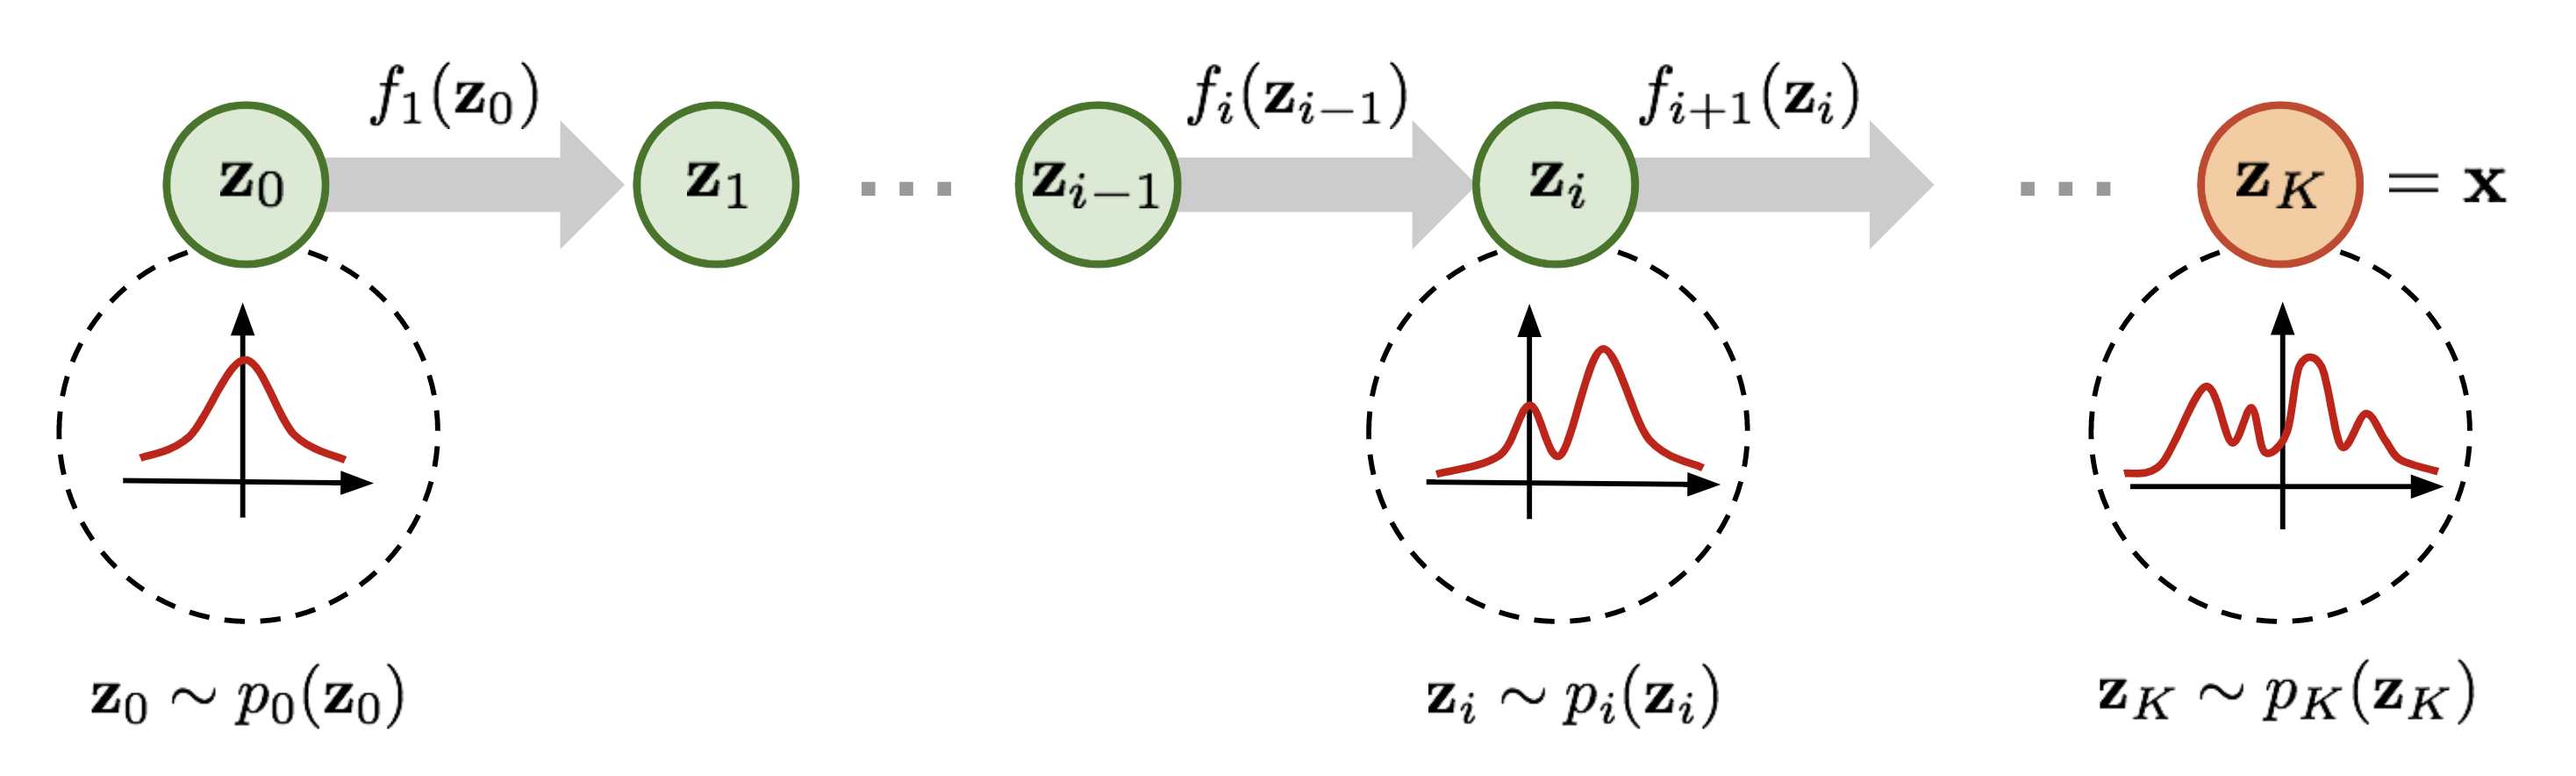
\includegraphics[scale=0.15]{ThuThesis_ Tsinghua University Thesis LaTeX Template/Picture/norm_flow.png}
    \caption{正则流图例}
    \label{Norm_flow}
\end{figure}
对于连续函数$f:\mathbb{R}^{d}\rightarrow \mathbb{R}^d$,其中$f$可逆,定义$f$逆映射$f^{-1}=g$,即$g\circ f(z)=z$。如果我们用该映射将具有密度函数$q(z)$的隐式随机变量$z$映射到$z^{\prime}=f(z)$,则$z'$有如下密度函数
\begin{equation}
    q(z^{\prime}) = q(z)|\operatorname{det}\frac{\partial f^{-1}}{\partial z^{\prime}}|= q(z)|\operatorname{det}\frac{\partial f}{\partial z}|^{-1},
    \label{chain rule}
\end{equation}
其中最后一个等式可以利用链式法则来进行推广(如果有多个函数复合的情况下),我们可以复合多个函数并且循环利用式(\ref{chain rule})。对于有$K$个映射作用下得到的随机变量$z_{K}$(如图\ref{Norm_flow}中所示),由随机变量$z_0$连续变换$K$次得到的随机变量的密度函数$q_{K}(z)$具有性质
\begin{equation}
    \ln q_{K}(z_{K}) = \ln q_{0}(z_0)-\sum_{k=1}^{K}\ln |\operatorname{det}\frac{\partial f_k}{\partial z_{k-1}}|
    \label{chain log likelihood}
\end{equation}
其中我们有
\begin{equation}
    z_{K}=f_{K}\circ \cdots f_1(z_0)
    \label{z_K definition}
\end{equation}
根据VAE模型的定义,我们的优化目标转换为如下目标:
\begin{equation}
    \ln p(\mathbf{x}) \geq \mathbb{E}_{q\left(\mathbf{z}^{(0)} \mid \mathbf{x}\right)}\left[\ln p\left(\mathbf{x} \mid \mathbf{z}^{(T)}\right)+\sum_{t=1}^T \ln \left|\operatorname{det} \frac{\partial \mathbf{f}^{(t)}}{\partial \mathbf{z}^{(t-1)}}\right|\right]-\mathrm{KL}\left(q\left(\mathbf{z}^{(0)} \mid \mathbf{x}\right) \| p\left(\mathbf{z}^{(T)}\right)\right)
    \label{NF objective}
    \end{equation}
正则流可以用来逼近不同类型的VAE模型中的后验分布,只需要选取合适的转换函数$f^{(t)}$,不需要对编码器和解码器的结构进行修改。在实际应用中,一般采取形式较为简单的可逆正则流(对每个元素进行运算而减少矩阵乘法的操作,从而不需要储存矩阵的逆提升计算速率)。以下列举代表性正则流例子。
\subsection{线性时间转换正则流模型(Invertible Linear-time Transformation)}
我们考虑如下形式的可逆变换
\begin{equation}
    f(z) = z+ u\cdot h(w^{\top } w + b)
    \label{family form}
\end{equation}
其中我们定义参数集$\lambda = \{w\in \mathbb{R}^{D}, u\in \mathbb{R}^D,b\in \mathbb{R}\}$ 为可以调节的参数,$h(\cdot)$为一个光滑非线性函数有导数$h'(\cdot)$,该映射对矩阵每一个元素进行相同的映射,为一个elementwise function。对于此类映射我们可以在$O(D)$复杂度时间内计算出对数雅可比项,计算如下
\begin{align}
    \psi(z) &= h'(w^{\top}z+b)w\\
    |\operatorname{det}\frac{\partial f}{\partial z}| &= |\operatorname{det}(I+u\cdot \psi(z)^{\top})|=|1+u^{\top}\psi(z)|
\end{align}
根据式(\ref{chain log likelihood})可以得到最终随机变量的似然函数以及根据在式(\ref{family form})中定义的正则流转换函数的形式可以得到在该族转换函数下的似然函数取值形式为
\begin{align}
     z_{K} &=f_{K}\circ \cdots f_1(z_0) \\
     \ln q_{K}(z_{K})&= \ln q_0(z)-\sum_{k=1}^{K}\ln |1+u_{k}^{\top}\psi_{k}(z_{k-1})|
\end{align}
\section{扩散模型}
扩散概率模型在图像生成领域已经被证明是有效的生成模型,但是其缺点在于缺乏低维的有效隐藏变量$z$。然而,VAE模型通常具有低维有效的隐藏变量,可以通过结合两者来更加有效地
获得对高维数据分布的逼近。
和VAE模型一样,扩散模型的目的也是希望能够学习得到目标高维样本的分布性质。 在\cite{diffusion}中详细讨论了扩散模型的性质并且介绍了扩散模型的特殊情况,即DDPM模型用来对实际应用中的高维数据进行处理。以下部分中,我们首先将对扩散模型的数学原理进行回顾。基于随机微分方程的背景,假设有一个如下的随机微分方程
\begin{equation}
    dz = f(t)\cdot z \rm{dt}+g(t)\rm{dw}.
    \label{SDE 1}
\end{equation}
其中$\{z_t\}_{t=0}^{t=1}$为一个正向的连续变化的扩散过程,其中$z_0$为初始的随机变量,在此处我们将其作为想要研究的为止分布,而$z_t$则为在$t$时刻扩散得到的随机变量。其中, $f: \mathbb{R}\rightarrow \mathbb{R}$与
 $g: \mathbb{R}\rightarrow \mathbb{R}$为一维函数,$w$为标准布朗运动。可以通过设计$f$和$g$使得$z_1$服从标准正态分布,即$z_1\sim \mathcal{N}(z_1;0,I)$。而在实际对该连续变化过程进行采样的时候,通常会使用Euler法,即将$[0,1]$区间分成$T$个子区间$[i/T,(i+1)/T], i =0,1,\cdots, (T-1)$, 仅关注每一个子区间端点处随机变量的分布,即为$z_{i/T},i=0,1,\cdots,T$。在\cite{diffusion}中已经证明在式(\ref{SDE 1})中的随机微分方程可以通过一个生成式模型从尾端进行反转。在该文章中,在保证$z_1$服从标准正态分布的前提假设下,可以先对$z_1\sim \mathcal{N}(z_1;0,I)$进行取样,其次对逆向随机微分方程 $dz = \left[f(t)\cdot z -g(t)^2 \nabla_z \log q_t(z)\right] \rm{dt} + g(t)d \Tilde{w}$进行求解。其中$\Tilde{w}$为逆向标准布朗运动。在该逆向随机微分方程中,需要知道$\nabla_z \log q_t(z)$,即为在$t$时刻随机变量的正向传播下的边缘分布的打分函数(score function)。
 在\cite{diffusion}中训练逆向传播过程的参数只需要最小化如下量用来匹配打分函数
\begin{equation}
    \min _{\boldsymbol{\theta}} \mathbb{E}_{t \sim \mathcal{U}[0,1]}\left[\lambda(t) \mathbb{E}_{q\left(\mathbf{z}_0\right)} \mathbb{E}_{q\left(\mathbf{z}_t \mid \mathbf{z}_0\right)}\left[|| \nabla_{\mathbf{z}_t} \log q\left(\mathbf{z}_t\right)-\nabla_{\mathbf{z}_t} \log p_{\boldsymbol{\theta}}\left(\mathbf{z}_t\right) \|_2^2\right]\right]
    \label{score objective 1}
\end{equation}
在此处我们还需要定义权重函数$\lambda(t)$。其中$q(z_0)$为目标样本的分布函数以及$q(z_t|z_0)$是扩散核,通过选取适当的$f(t)$和$g(t)$可以使得$q(z_t|z_0)$有解析表达式。在一般设定下由于不能保证有解析表达式,在\cite{diffusion}中将式(\ref{score objective 1})转换为优化如下目标
\begin{equation}
    \min _{\boldsymbol{\theta}} \mathbb{E}_{t \sim \mathcal{U}[0,1]}\left[\lambda(t) \mathbb{E}_{q\left(\mathbf{z}_0\right)} \mathbb{E}_{q\left(\mathbf{z}_t \mid \mathbf{z}_0\right)}\left[|| \nabla_{\mathbf{z}_t} \log q\left(\mathbf{z}_t \mid \mathbf{z}_0\right)-\left.\nabla_{\mathbf{z}_t} \log p_{\boldsymbol{\theta}}\left(\mathbf{z}_t\right)\right|_2 ^2\right]\right]+C
    \label{score objective 2}
\end{equation}
其中$C=\mathbb{E}_{t \sim \mathcal{U}[0,1]}\left[\lambda(t) \mathbb{E}_{q\left(\mathbf{z}_0\right)} \mathbb{E}_{q\left(\mathbf{z}_t \mid \mathbf{z}_0\right)}\left[\left\|\nabla_{\mathbf{z}_t} \log q\left(\mathbf{z}_t\right)\right\|_2^2-\left\|\nabla_{\mathbf{z}_t} \log q\left(\mathbf{z}_t \mid \mathbf{z}_0\right)\right\|_2^2\right]\right]$,在
\cite{vincent}中说明了$C$的取值不取决于$\theta$,因此由式(\ref{score objective 2})和式(\ref{score objective 1})优化得到的参数$\theta$是等价的。为了计算上的便捷,通常会取$\lambda(t) = g(t)^2/2$, 其中在\cite{song_2}中说明了如果以如上方式选取权重函数$\lambda(t)$则可以使得在KL-散度意义下的目标分布和逆向SDE生成的分布的距离可以以式(\ref{score objective 1})作为上界,即
\begin{equation}
\operatorname{KL}\left(q\left(\mathbf{z}_0\right) \| p_{\boldsymbol{\theta}}\left(\mathbf{z}_0\right)\right) \leq \mathbb{E}_{t \sim \mathcal{U}[0,1]}\left[\frac{g(t)^2}{2} \mathbb{E}_{q\left(\mathbf{z}_0\right)} \mathbb{E}_{q\left(\mathbf{z}_t \mid \mathbf{z}_0\right)}\left[\left\|\nabla_{\mathbf{z}_t} \log q\left(\mathbf{z}_t\right)-\nabla_{\mathbf{z}_t} \log p_{\boldsymbol{\theta}}\left(\mathbf{z}_t\right)\right\|_2^2\right]\right]
    \label{KL upper bound 1}
\end{equation}
在实际优化模型中,只需要对式(\ref{score objective 2})进行最小化即可,在得到相应模型参数$\theta$后对逆向随机微分方程进行求解可以得到对目标分布的逼近。由于扩散模型只需要保证末端的随机变量$z_1$服从正态分布,因此可以选取不同的$f(t)$,$g(t)$函数来生成目标分布。在接下来的部分中将着重分析一类特殊的扩散模型:DDPM模型。(Denoising Diffusion Probabilistic Models)
\section{降噪扩散概率模型(DDPM)}
在本部分将重新引入新的符号,这里我们定义$x_i= z_{i/T},i=0,1,\cdots,T$。
扩散模型为隐式变量模型满足如下形式$p_{\theta}(x_0) = \int p_{\theta}(x_{0:T}) dx_{1:T}$。其中$x_0=z_0\sim q(z_0)$为样本中的原始分布,$x_1,\cdots, x_{T}$ 为和$x_0$相同维数的隐式变量。 $x_T$对应一般扩散模型中的$z_1$,满足服从标准正态分布。由于$x_{0:T}$分别对应在$[0,1]$区间中的通过Euler法得到格点上的随机变量,由于此处可以假设$T$足够大,因此每一个相邻的条件概率分布$q(x_{i+1}|x_i)$都服从正态分布(利用布朗运动的性质)。\par 
首先开始定义正向过程,在正向过程中,扩散模型采用一步步向样本增加白噪声的方式,使得最终获得的随机变量$x_T$的分布趋近于正态分布。我们在此处通过选取参数$\beta_1, \cdots, \beta_{T}$ 的方式来选取每次增加噪声的大小。扩散模型的目的在于先用正向过程从$x_0$过渡到$x_T$使得其分布趋近于正态分布,再利用参数化得到的逆向过程来生成对初始样本分布的逼近。仿照逆向过程联合分布函数,正向联合分布函数的形式可以写为如下的形式:($\beta_t$用来定义相邻的条件概率分布的参数)
\begin{equation}
    q\left(x_{1: T} \mid x_0\right)=\prod_{t=1}^T q\left(x_t \mid x_{t-1}\right)
    \end{equation}
    \begin{equation}
        q\left(x_t \mid x_{t-1}\right)=\mathcal{N}\left(\sqrt{1-\beta_t} x_{t-1}, \beta_t I\right)
        \end{equation}
        \begin{equation}
            q\left(x_t \mid x_0\right)=\mathcal{N}\left(\sqrt{\bar{\alpha}_t} x_0,\left(1-\overline{\alpha_t}\right) I\right) \text { 其中 } \alpha_t=\left(1-\beta_t\right) \text { 以及 } \bar{\alpha}_t=\prod_t \alpha_t
            \label{posterior of xt}
            \end{equation}
    正向传播的后验分布同样可以被给出:
    \begin{equation}
        q\left(x_{t-1} \mid x_t, x_0\right)=\mathcal{N}\left(\tilde{\mu}_t\left(x_t, x_0\right), \tilde{\beta}_t\right)
        \label{posterior xt 2}
        \end{equation}
        \begin{equation}
            \text {     其中 } \tilde{\mu}_t\left(x_t, x_0\right)=\frac{\sqrt{\bar{\alpha}_{t-1}} \beta_t}{1-\bar{\alpha}_t} x_0+\frac{\sqrt{\alpha_t}\left(1-\bar{\alpha}_{t-1}\right)}{1-\bar{\alpha}_t} x_t
            \end{equation}
            \begin{equation}
                \text { 以及 } \quad \tilde{\beta}_t=\frac{1-\bar{\alpha}_{t-1}}{1-\bar{\alpha}_t} \beta_t
                \end{equation}
该正向过程实际上对应的随机微分方程即为
\begin{equation}
    dz = -\frac{g(t)^2}{2}\cdot  z dt + g(t)dw
\end{equation}
$x_{0:T}$的联合分布$p_{\theta}(x_{0:T})$被称为逆向过程,并且它被定义为一个Markov过程,该过程的转移分布可以从末端$p(x_T)= \mathcal{N}(x_T;0,I) $开始。由此可以写出逆向过程的联合分布函数的表达式
\begin{equation}
    p_{\theta}(x_{0:T}) := p(x_T)\prod_{t=1}^{T}p_{\theta}(x_{t-1}|x_t), p_{\theta}(x_{t-1}|x_t) :=\mathcal{N}(x_{t-1};\mu_{\theta}(x_t,t),\Sigma_{\theta}(x_t,t)).  
\end{equation}

以上为正向Markov过程所满足的条件概率分布性质,在随机优化问题中为了优化参数需要对逆向传播过程进行建模。
逆向传播过程同样可以被参数化,此处使用高斯转移分布来进行此一阶Markov逆向传播过程,满足如下表达式:
\begin{equation}
    p\left(x_{0: T}\right)=p\left(x_T\right) \prod_{t=1}^T p_\theta\left(x_{t-1} \mid x_t\right)
    \end{equation}
    \begin{equation}
        p_\theta\left(x_{t-1} \mid x_t\right)=\mathcal{N}\left(\mu_\theta\left(x_t, t\right), \Sigma_\theta\left(x_t, t\right)\right)
        \end{equation}
        \begin{figure}[H]
            \centering
            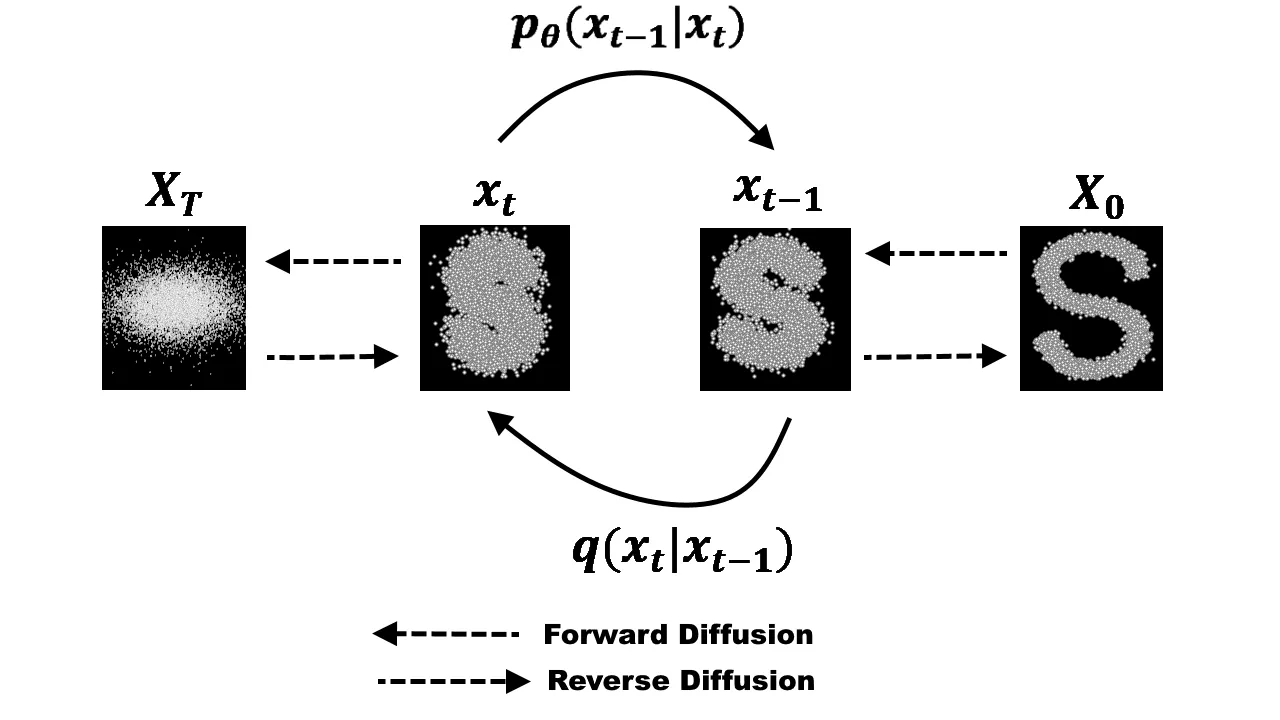
\includegraphics[scale = 0.2]{ThuThesis_ Tsinghua University Thesis LaTeX Template/Picture/Diffusion.png}
            \caption{扩散模型图例}
            \label{Diffusion}
        \end{figure}
选取足够大的$T$值与合适的递减序列$\{\beta_t\}_{t\geq 1}$, 条件概率分布$q(x_{T}|x_0)$可以足够接近标准高斯分布。
整个概率系统可以通过变分推断来进行端到端的训练,从而优化参数。
在该模型下,同样采用极大似然估计的方式来进行参数优化,此处采用最大化对数似然函数的相反数的上界来进行优化,即
\begin{equation}
    \mathbb{E}\left[-\log p_\theta\left(\mathbf{x}_0\right)\right] \leq \mathbb{E}_q\left[-\log \frac{p_\theta\left(\mathbf{x}_{0: T}\right)}{q\left(\mathbf{x}_{1: T} \mid \mathbf{x}_0\right)}\right]=\mathbb{E}_q\left[-\log p\left(\mathbf{x}_T\right)-\sum_{t \geq 1} \log \frac{p_\theta\left(\mathbf{x}_{t-1} \mid \mathbf{x}_t\right)}{q\left(\mathbf{x}_t \mid \mathbf{x}_{t-1}\right)}\right]=: L
    \label{DDPM objective 1}
\end{equation}
从随机优化方法的角度去考虑,可以将式(\ref{DDPM objective 1})重新写为
\begin{equation}
\mathbb{E}_q[\underbrace{\mathcal{D}_{K L}\left(q\left(x_T \mid x_0\right) \| p\left(x_T\right)\right)}_{L_T}+\sum_{t>1} \underbrace{\mathcal{D}_{K L}\left(q\left(x_{t-1} \mid x_t, x_0\right) \| p_\theta\left(x_{t-1} \mid x_t\right)\right)}_{L_{t-1}}-\underbrace{\log p_\theta\left(x_0 \mid x_1\right)}_{L_0}]
    \end{equation}
以上为DDPM的数学原理,以下将具体讨论DDPM在实际优化过程中的参数设计与模型细节。以上已经将$L$分解成$L_T,L_{t-1},L_0$三大部分,由于后验分布$q$没有任何参数,因此$L_T$可以直接忽略(和$\theta$取值近似无关)。
在\cite{DDPM}中直接假设$\Sigma_{\theta}(x_t,t)=\sigma_t^2 I$,方便简化计算过程(避免矩阵求逆运算操作)。其次,为了表示$\mu_{\theta}(x_t,t)$,由于$p_{\theta}(x_{t-1}|x_t):= \mathcal{N}(x_{t-1};\mu_{\theta}(x_t,t),\sigma_t^2I)$,我们可以将$L_{t-1}$写为
\begin{equation}
    L_{t-1}=\mathbb{E}_q\left[\frac{1}{2 \sigma_t^2}\left\|\tilde{\boldsymbol{\mu}}_t\left(\mathbf{x}_t, \mathbf{x}_0\right)-\boldsymbol{\mu}_\theta\left(\mathbf{x}_t, t\right)\right\|^2\right]+C
    \label{Lt representation}
\end{equation}
其中$C$为一个和$\theta$无关的常数,在优化过程中可以被忽略。利用式(\ref{posterior of xt})可以进一步简化式(\ref{Lt representation}) 将$x_t$表示为$\mathbf{x}_t\left(\mathbf{x}_0, \boldsymbol{\epsilon}\right)=\sqrt{\bar{\alpha}_t} \mathbf{x}_0+\sqrt{1-\bar{\alpha}_t} \boldsymbol{\epsilon} \text { for } \boldsymbol{\epsilon} \sim \mathcal{N}(\mathbf{0}, \mathbf{I}) $, 以及利用式(\ref{posterior xt 2})可以得到
\begin{align}
    L_{t-1}-C&=\mathbb{E}_{\mathbf{x}_0, \boldsymbol{\epsilon}}\left[\frac{1}{2 \sigma_t^2}\left\|\tilde{\boldsymbol{\mu}}_t\left(\mathbf{x}_t\left(\mathbf{x}_0, \boldsymbol{\epsilon}\right), \frac{1}{\sqrt{\bar{\alpha}_t}}\left(\mathbf{x}_t\left(\mathbf{x}_0, \boldsymbol{\epsilon}\right)-\sqrt{1-\bar{\alpha}_t} \boldsymbol{\epsilon}\right)\right)-\boldsymbol{\mu}_\theta\left(\mathbf{x}_t\left(\mathbf{x}_0, \boldsymbol{\epsilon}\right), t\right)\right\|^2\right]\\
&=\mathbb{E}_{\mathbf{x}_0, \boldsymbol{\epsilon}}\left[\frac{1}{2 \sigma_t^2}\left\|\frac{1}{\sqrt{\alpha_t}}\left(\mathbf{x}_t\left(\mathbf{x}_0, \boldsymbol{\epsilon}\right)-\frac{\beta_t}{\sqrt{1-\bar{\alpha}_t}} \boldsymbol{\epsilon}\right)-\boldsymbol{\mu}_\theta\left(\mathbf{x}_t\left(\mathbf{x}_0, \boldsymbol{\epsilon}\right), t\right)\right\|^2\right]
\end{align}
\section{去噪扩散隐式模型(DDIM)}
在DDPM的基础上,针对原模型所存在的缺陷,提出了DDIM,即去噪扩散隐式模型。在\cite{DDIM}中,针对DDPM所存在的缺陷,即每次进行优化需要生成整条Markov链需要较大计算复杂度的缺陷,提出了DDIM,即通过非Markov过程生成整条链。通过对比DDIM和DDPM的训练效果,发现DDIM可以生成更高质量的图像。接下来详细阐述DDIM模型正向生成样本的过程。
在正向传播过程中,Markov链的似然函数可以被写成如下形式:
\begin{equation}
    q_\sigma\left(\boldsymbol{x}_{1: T} \mid \boldsymbol{x}_0\right):=q_\sigma\left(\boldsymbol{x}_T \mid \boldsymbol{x}_0\right) \prod_{t=2}^T q_\sigma\left(\boldsymbol{x}_{t-1} \mid \boldsymbol{x}_t, \boldsymbol{x}_0\right)
\end{equation}
其中我们还有 $q_\sigma\left(\boldsymbol{x}_T \mid \boldsymbol{x}_0\right)=\mathcal{N}\left(\sqrt{\alpha_T} \boldsymbol{x}_0,\left(1-\alpha_T\right) \boldsymbol{I}\right)$ 以及对与所有的$t>1$,我们还有
$$
q_\sigma\left(\boldsymbol{x}_{t-1} \mid \boldsymbol{x}_t, \boldsymbol{x}_0\right)=\mathcal{N}\left(\sqrt{\alpha_{t-1}} \boldsymbol{x}_0+\sqrt{1-\alpha_{t-1}-\sigma_t^2} \cdot \frac{\boldsymbol{x}_t-\sqrt{\alpha_t} \boldsymbol{x}_0}{\sqrt{1-\alpha_t}}, \sigma_t^2 \boldsymbol{I}\right)
$$
以及对于每个$t$,可以选择合适的均值函数,使得$q_\sigma\left(\boldsymbol{x}_t \mid \boldsymbol{x}_0\right)=\mathcal{N}\left(\sqrt{\alpha_t} \boldsymbol{x}_0,\left(1-\alpha_t\right) \boldsymbol{I}\right)$。
根据贝叶斯公式,我们可以得到实际的条件分布密度函数为
\begin{equation}
   q_\sigma\left(\boldsymbol{x}_t \mid \boldsymbol{x}_{t-1}, \boldsymbol{x}_0\right)=\frac{q_\sigma\left(\boldsymbol{x}_{t-1} \mid \boldsymbol{x}_t, \boldsymbol{x}_0\right) q_\sigma\left(\boldsymbol{x}_t \mid \boldsymbol{x}_0\right)}{q_\sigma\left(\boldsymbol{x}_{t-1} \mid \boldsymbol{x}_0\right)}
   \label{Bayes Formula 1}
\end{equation}
根据式(\ref{Bayes Formula 1})可以得到如上分布依然为高斯分布。在该正向生成过程中,该链已经不满足Markov性质了。每次通过$\boldsymbol{x}_t,\boldsymbol{x}_0$生成$\boldsymbol{x}_{t+1}$。接下来阐述反向传播链条的具体表达形式。首先,基于$\boldsymbol{x}_t$可以得到对于$\boldsymbol{x}_0$的一个估计,其次再利用两者的结合去预测$\boldsymbol{x}_{t-1}$。对于某个$\boldsymbol{x}_0\sim q(\boldsymbol{x}_0)$以及$\epsilon_t \sim \mathcal{N}(0,I)$,函数$\epsilon_{\theta}^{(t)}(\boldsymbol{x}_t)$旨在通过$\boldsymbol{x}_t$去预测$\epsilon_t$。通过函数$f^{(t)}_{\theta}$来进行对$\boldsymbol{x}_0$的预测。
\begin{equation}
f_\theta^{(t)}\left(\boldsymbol{x}_t\right):=\left(\boldsymbol{x}_t-\sqrt{1-\alpha_t} \cdot \epsilon_\theta^{(t)}\left(\boldsymbol{x}_t\right)\right) / \sqrt{\alpha_t}.
\end{equation}
如下可以定义反向传播过程,
\begin{equation}
 p_\theta^{(t)}\left(\boldsymbol{x}_{t-1} \mid \boldsymbol{x}_t\right)= \begin{cases}\mathcal{N}\left(f_\theta^{(1)}\left(\boldsymbol{x}_1\right), \sigma_1^2 \boldsymbol{I}\right) & \text { if } t=1 \\ q_\sigma\left(\boldsymbol{x}_{t-1} \mid \boldsymbol{x}_t, f_\theta^{(t)}\left(\boldsymbol{x}_t\right)\right) & \text { 其余情形 }\end{cases}   
\end{equation}
通过变分推断的技术,可以计算得到ELBO的值,最后可以通过优化如下目标来得到参数$\theta$
\begin{align} & J_\sigma\left(\epsilon_\theta\right):=\mathbb{E}_{\boldsymbol{x}_{0: T} \sim q_\sigma\left(\boldsymbol{x}_{0: T}\right)}\left[\log q_\sigma\left(\boldsymbol{x}_{1: T} \mid \boldsymbol{x}_0\right)-\log p_\theta\left(\boldsymbol{x}_{0: T}\right)\right] \\ = & \mathbb{E}_{\boldsymbol{x}_{0: T} \sim q_\sigma\left(\boldsymbol{x}_{0: T}\right)}\left[\log q_\sigma\left(\boldsymbol{x}_T \mid \boldsymbol{x}_0\right)+\sum_{t=2}^T \log q_\sigma\left(\boldsymbol{x}_{t-1} \mid \boldsymbol{x}_t, \boldsymbol{x}_0\right)-\sum_{t=1}^T \log p_\theta^{(t)}\left(\boldsymbol{x}_{t-1} \mid \boldsymbol{x}_t\right)-\log p_\theta\left(\boldsymbol{x}_T\right)\right]\end{align}
在实际优化中,不需要每次生成T个样本,可以只选取部分样本根据条件概率分布进行生成再进行优化。
(可以参考DDIM中的accleration部分)
\section{VAE模型和扩散模型的结合:隐式扩散模型}
结合扩散模型的优点,可以去除在VAE模型中隐式变量$z$的先验分布为标准正态分布的假设。在得到隐式变量$z$后,先通过一个扩散模型学习到$p_{\theta}(z_0)$用来逼近$z_0$的真实分布,然后再通过解码器生成$x$的分布。接下来我们对该混合模型的原理进行具体回顾,在\cite{VAE_diffusion}中对该方法进行了详细的阐述。对于传统VAE模型,隐含假设为隐式变量$z$的先验分布为标准正态分布,然而该假设对于现实生活中许多具有离散分布的数据并不成立。因此需要通过扩散模型去学习到真实的隐式变量的分布,接下来详细说明该模型的执行流程。
在该模型下,我们依然只考虑如下形式的随机微分方程进行扩散
\begin{equation}
    dz = f(t)\cdot zdt + g(t)dW_t
    \label{SDE form }
\end{equation}
其中$\{W_t\}_{t\geq 0}$为标准布朗运动
\begin{figure}[H]
    \centering
    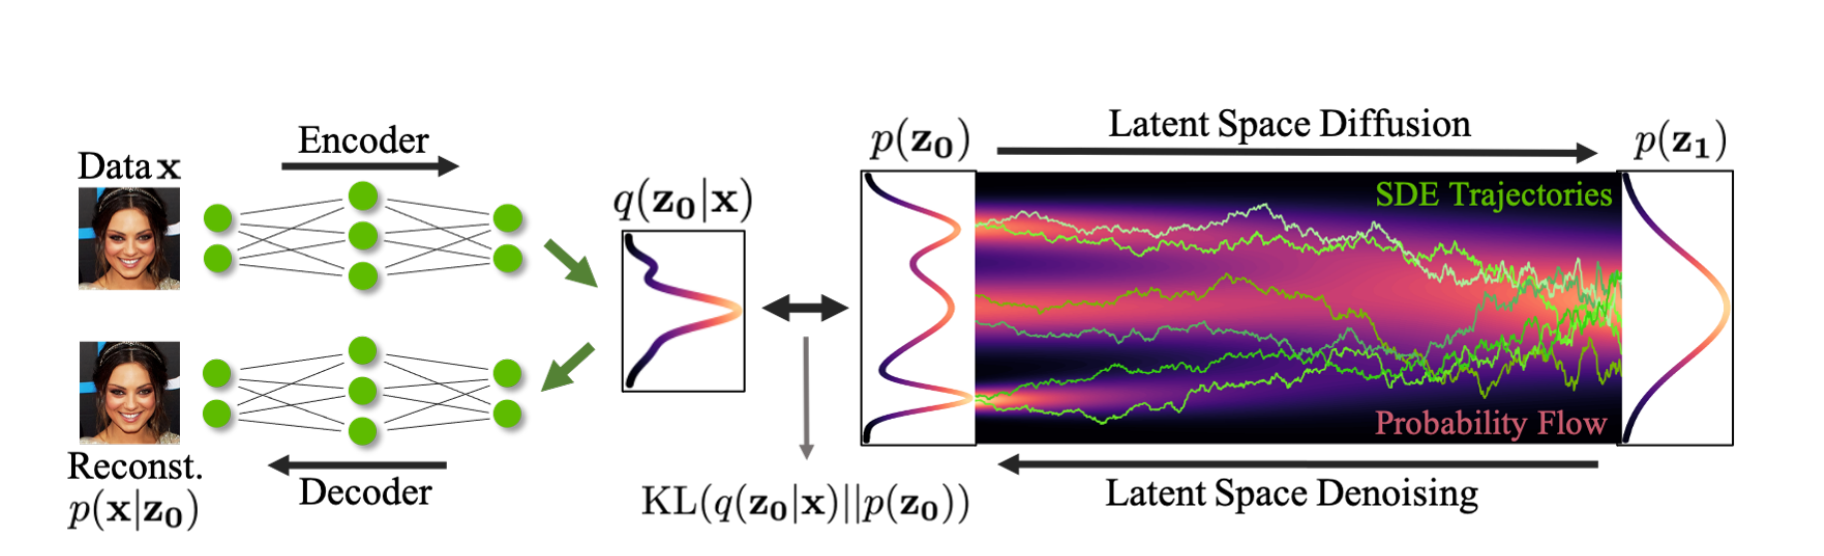
\includegraphics[scale = 0.5]{ThuThesis_ Tsinghua University Thesis LaTeX Template/Picture/VAE_diffusion.png}
    \caption{VAE模型和扩散模型的结合}
    \label{fig_VAE_Diffusion}
\end{figure}
在图\ref{fig_VAE_Diffusion}中,由三部分组成:编码器$q_{\phi}(z_0|x)$, 扩散模型$p_{\theta}(z_0)$和解码器$p_{\psi}(x|z_0)$。首先样本$x$利用编码器得到隐式变量$z_0$,再通过扩散模型通过$z_0$扩散到$z_1$使得$z_1$服从标准正态分布$z_1\sim \mathcal{N}(z_1;0,I)$。利用逆向微分方程可以从末端$z_1$开始取样通过解方程采样得到$z_0$的分布的近似$p_{\theta}(z_0)$。最后,通过解码器可以通过$p_{\psi}(x|z_0)$将隐式变量映射到原先的样本空间中。在该模型中,和VAE模型的处理方法相同,我们依然通过极大似然估计的方法去进行参数训练。我们在此处最小化对数似然函数相反数的下界(ELBO)来进行参数估计,
\begin{align}
 \mathcal{L}(\mathbf{x}, \boldsymbol{\phi}, \boldsymbol{\theta}, \boldsymbol{\psi})&=\mathbb{E}_{q_{\boldsymbol{\phi}}\left(\mathbf{z}_0 \mid \mathbf{x}\right)}\left[-\log p_{\boldsymbol{\psi}}\left(\mathbf{x} \mid \mathbf{z}_0\right)\right]+\operatorname{KL}\left(q_{\boldsymbol{\phi}}\left(\mathbf{z}_0 \mid \mathbf{x}\right) \| p_{\boldsymbol{\theta}}\left(\mathbf{z}_0\right)\right) \label{Loss decomposition 1}\\
& =\underbrace{\mathbb{E}_{q_{\boldsymbol{\phi}}\left(\mathbf{z}_0 \mid \mathbf{x}\right)}\left[-\log p_{\boldsymbol{\psi}}\left(\mathbf{x} \mid \mathbf{z}_0\right)\right]}_{\text {reconstruction term }}+\underbrace{\mathbb{E}_{q_\phi\left(\mathbf{z}_0 \mid \mathbf{x}\right)}\left[\log q_{\boldsymbol{\phi}}\left(\mathbf{z}_0 \mid \mathbf{x}\right)\right]}_{\text {negative encoder entropy }}+\underbrace{\mathbb{E}_{q_{\boldsymbol{\phi}}\left(\mathbf{z}_0 \mid \mathbf{x}\right)}\left[-\log p_{\boldsymbol{\theta}}\left(\mathbf{z}_0\right)\right]}_{\text {cross entropy }} \label{loss decomposition 2}
\end{align}
通过式(\ref{loss decomposition 2})可以将式(\ref{Loss decomposition 1})中的KL散度进行进一步分解。在式(\ref{loss decomposition 2})中的reconstruction term 和 encoder entropy term都可以通过VAE模型中所使用的重参数化技巧来进行估计优化,在优化中最困难的部分是对交叉熵部分进行估计求导。以下引用在\cite{VAE_diffusion}中得到的关于交叉熵的结论。
\begin{theorem}
在随机微分方程式(\ref{SDE form })下,考虑两个初始分布$q(z_0)$和$p(z_0)$,都定义在$\mathbb{R}^{D}$上,假设$q(z_t)$ ,$p(z_t)$代表在SDE(\ref{SDE form })下在$t\in [0,1]$时刻扩散得到的随机变量的边缘分布。同时假设$\log(p(z_t))$和$\log(q(z_t))$均为光滑函数且在$z_t\to \infty$时增长速度不超过多项式量级增长。同时我们假设所选取的$f(t)$
$g(t)$满足在$t=1$时刻满足$q(z_1)=p(z_1)$,则交叉熵满足以下等式
\begin{align}
    \operatorname{CE}\left(q\left(\mathbf{z}_0 \mid \mathbf{x}\right) \| p\left(\mathbf{z}_0\right)\right) &=\mathbb{E}_{t \sim \mathcal{U}[0,1]}\left[\frac{g(t)^2}{2} \mathbb{E}_{q\left(\mathbf{z}_t, \mathbf{z}_0 \mid \mathbf{x}\right)}\left[\left\|\nabla_{\mathbf{z}_t} \log q\left(\mathbf{z}_t \mid \mathbf{z}_0\right)-\nabla_{\mathbf{z}_t} \log p\left(\mathbf{z}_t\right)\right\|_2^2\right]\right] \nonumber\\
    &+\frac{D}{2} \log \left(2 \pi e \sigma_0^2\right) \label{thm 1}
\end{align}
    其中$q(z_t,z_0|x) = q(z_t|z_0)q(z_0|x)$,以及条件概率分布$q(z_t|z_0)$为正态分布有如下形式$q(z_t|z_0)=\mathcal{N}(z_t;\mu_t(z_0),\sigma_t^2)$。其中$\mu_t$,$\sigma_t^2$由$f(t)$和$g(t)$以及初始时刻$t=0$处方差$\sigma_0^2$唯一确定。
\end{theorem}
根据以上结论,在实际优化过程中需要对$t$时刻的随机变量$z_t$进行采样来进行随机梯度下降,然而根据该种采样得到的随机变量可能有较高的方差,在实际优化中需要采用一定的减小采样方差的方法。 在实际应用中通常会对VPSDE(Variance Preserving SDE)进行分析,即SDE形式为
\begin{equation}
    dz = -\frac{1}{2}\beta(t)zdt + \sqrt{\beta(t)}dW.
    \label{VPSDE}
\end{equation}
其中我们可以定义$\beta(t) = \beta_0+(\beta_1-\beta_0)t$,从而使得该函数取值始终在$[\beta_0,\beta_1]$内。(也可以更换该函数形式满足更加复杂的应用需求)
在\cite{Consistency}中对一致性模型的诸多性质进行了详细的阐述。\par 
在实际应用中,由于图像的维数相对较高,如果直接使用Diffusion Model进行训练(例如使用DDPM等模型)会带来较大的计算资源消耗,因此通常会先将图像通过编码器映射到隐空间中,通过Diffusion Model训练得到隐空间变量的真实分布,最后再通过解码器得到还原后的图像。该方法可以用于图像去噪,图像生成等下游任务。在\cite{High_synthesis}中详细阐述了使用VAE模型和Diffusion Model的结合在图像生成中的丰富应用。以及如果再充分使用Transformer模型,可以进一步实现文字转图像等丰富功能。
% \chapter{研究问题简述}
本文的主要研究问题为对目标图像进行去噪处理,得到相应去噪前的可能图像的生成。首先回顾传统生成模型的适用条件与背景。传统的扩散模型,如\cite{song_2,DDPM,DDIM}中的扩散模型,均用于实现从纯噪声图片生成原图像分布。其中最关键的步骤为Score-matching, 即为通过参数拟合学习得到真实的对数密度函数的梯度。即假设原定未知目标分布为$X_0\sim p(X_0)$, 通过构造扩散过程得到随机过程$X_{0:T}$使得$p(X_{T})\sim \mathcal{N}(0,I)$(或者使得分布趋近于标准正态分布即可)。 Score-matching即为,在选取较大的$T$的情况下,学到$\nabla_{X_t}\log (p(X_t))$的值,记该函数为Score-function。     

在\cite{song_2}中主要采用解逆向随机微分方程来获得对目标未知分布的一个采样。问题设定主要如下:   

目标未知分布为$p(x_0)$,通过构造扩散过程
\begin{equation}
    dx = f(x,t)dt + g(t)dW_t,
    \label{diffusion equation SDE 1}
\end{equation}
其中$W_t$为标准的布朗运动,以$x_0$为初始随机变量,实际通过欧拉法离散化生成$x_{i/T}$, $i=1,\cdots, T$, 最后采样得到$x_1$。通过设计特定形式的随机微分方程(\ref{diffusion equation SDE 1}),可以使得最终随机变量$x_1$的概率分布为形式较为简单的概率分布 (例如为标准高斯分布)。   

在已知(\ref{diffusion equation SDE 1}) 的形式的情形下,存在以$x_1$为初始值的逆向随机微分方程
\begin{equation}
     dx = \left(f(x,t)-g^2(t)\nabla_{x_t}\log(q_t(x_t))\right)dt + g(t)d\Tilde{w}_t,
    \label{reverse diffusion equation SDE 1}
\end{equation}
因此只需要得到打分函数(Score function)的信息,即可从$x_1$开始逆向利用欧拉法进行离散化取样,当步长$T$足够大的时候,则离散化间距$1/T$足够小, 根据 
\cite{detemple}中对于Monte Carlo Estimator的渐进性质的分析,在使用Euler 法进行离散化取样的时候可以以$1/\sqrt{T}$的收敛速度趋近真实随机变量的分布;当采用Doss Transformation使得随机变量的随机微分方程的Diffusion 项为非随机量的时候,则可以以$1/T$的速率分布上收敛至真实分布。考虑到(\ref{diffusion equation SDE 1})的形式,通常取$T=1000$量级的步长已经可以有较好的逼近效果。      

由于在(\ref{reverse diffusion equation SDE 1})中唯一的位置量即为目标函数Score function $\nabla_{x_t}\log(q_t(x_t))$, 可以用一个和时间和随机变量本身相关的函数$S_{\theta}(t,x)$ 来逼近,其中$\theta$为该函数的参数化。具体优化参数的方式即为
\begin{equation}
{\theta}^*=\underset{{\theta}}{\arg \min } \mathbb{E}_t\left\{\lambda(t) \mathbb{E}_{\mathbf{x}(0)} \mathbb{E}_{\mathbf{x}(t) \mid \mathbf{x}(0)}\left[\left\|\mathbf{s}_{{\theta}}(\mathbf{x}(t), t)-\nabla_{\mathbf{x}(t)} \log p_{0 t}(\mathbf{x}(t) \mid \mathbf{x}(0))\right\|_2^2\right]\right\},
\label{score matching}
\end{equation}
其中$\lambda(t)$, $t\in [0,1]$为设置的权重函数,旨在使得优化得到的权重函数不仅仅在优化某些特定时刻的误差。优化得到最佳的打分函数Score function 的优化过程 (\ref{score matching}) 即为Score matching。    


根据\cite{score_based_SDE}中通过解逆向随机微分方程的想法,可以通过设计不同的随机微分方程形式来得到不同的采样方式,以及可以设计不同的正向采样和逆向采样算法,可以让生成方式为Markovian的也可以为Non-Markovian的。在\cite{DDPM}中设计了一种特定的随机微分方程来进行采样生成,方程满足如下形式。
\begin{equation}
    dz = -\left(\beta(t)/2\right)z dt + \sqrt{\beta(t)}dW_t,
    \label{DDPM Equation}
\end{equation}
在进行离散化取样生成正向传播链的时候,可以表达为目标分布为$x_0$,从$x_0$开始正向传播生成$x_{1:T}$, 满足条件概率分布为
\begin{equation}
    q\left(x_{1: T} \mid x_0\right)=\prod_{t=1}^T q\left(x_t \mid x_{t-1}\right)
    \end{equation}
    \begin{equation}
        q\left(x_t \mid x_{t-1}\right)=\mathcal{N}\left(\sqrt{1-\beta_t} x_{t-1}, \beta_t I\right)
        \end{equation}
        \begin{equation}
            q\left(x_t \mid x_0\right)=\mathcal{N}\left(\sqrt{\bar{\alpha}_t} x_0,\left(1-\overline{\alpha_t}\right) I\right) \text { 其中 } \alpha_t=\left(1-\beta_t\right) \text { 以及 } \bar{\alpha}_t=\prod_t \alpha_t
            \label{posterior of xt}
            \end{equation}
    正向传播的后验分布同样可以被给出:
    \begin{equation}
        q\left(x_{t-1} \mid x_t, x_0\right)=\mathcal{N}\left(\tilde{\mu}_t\left(x_t, x_0\right), \tilde{\beta}_t\right)
        \label{posterior xt 2}
        \end{equation}
        \begin{equation}
            \text {     其中 } \tilde{\mu}_t\left(x_t, x_0\right)=\frac{\sqrt{\bar{\alpha}_{t-1}} \beta_t}{1-\bar{\alpha}_t} x_0+\frac{\sqrt{\alpha_t}\left(1-\bar{\alpha}_{t-1}\right)}{1-\bar{\alpha}_t} x_t
            \end{equation}
            \begin{equation}
                \text { 以及 } \quad \tilde{\beta}_t=\frac{1-\bar{\alpha}_{t-1}}{1-\bar{\alpha}_t} \beta_t
                \end{equation}
该正向过程实际上对应的随机微分方程即为
\begin{equation}
    dz = -\frac{g(t)^2}{2}\cdot  z dt + g(t)dw
\end{equation}
$x_{0:T}$的联合分布$p_{\theta}(x_{0:T})$被称为逆向过程,并且它被定义为一个Markov过程,该过程的转移分布可以从末端$p(x_T)= \mathcal{N}(x_T;0,I) $开始。由此可以写出逆向过程的联合分布函数的表达式
\begin{equation}
    p_{\theta}(x_{0:T}) := p(x_T)\prod_{t=1}^{T}p_{\theta}(x_{t-1}|x_t), p_{\theta}(x_{t-1}|x_t) :=\mathcal{N}(x_{t-1};\mu_{\theta}(x_t,t),\Sigma_{\theta}(x_t,t)).  
\end{equation}

以上为正向Markov过程所满足的条件概率分布性质,在随机优化问题中为了优化参数需要对逆向传播过程进行建模。
逆向传播过程同样可以被参数化,此处使用高斯转移分布来进行此一阶Markov逆向传播过程,满足如下表达式:
\begin{equation}
    p\left(x_{0: T}\right)=p\left(x_T\right) \prod_{t=1}^T p_\theta\left(x_{t-1} \mid x_t\right)
    \end{equation}
    \begin{equation}
        p_\theta\left(x_{t-1} \mid x_t\right)=\mathcal{N}\left(\mu_\theta\left(x_t, t\right), \Sigma_\theta\left(x_t, t\right)\right)
        \end{equation}
        % \begin{figure}[H]
        %     \centering
        %     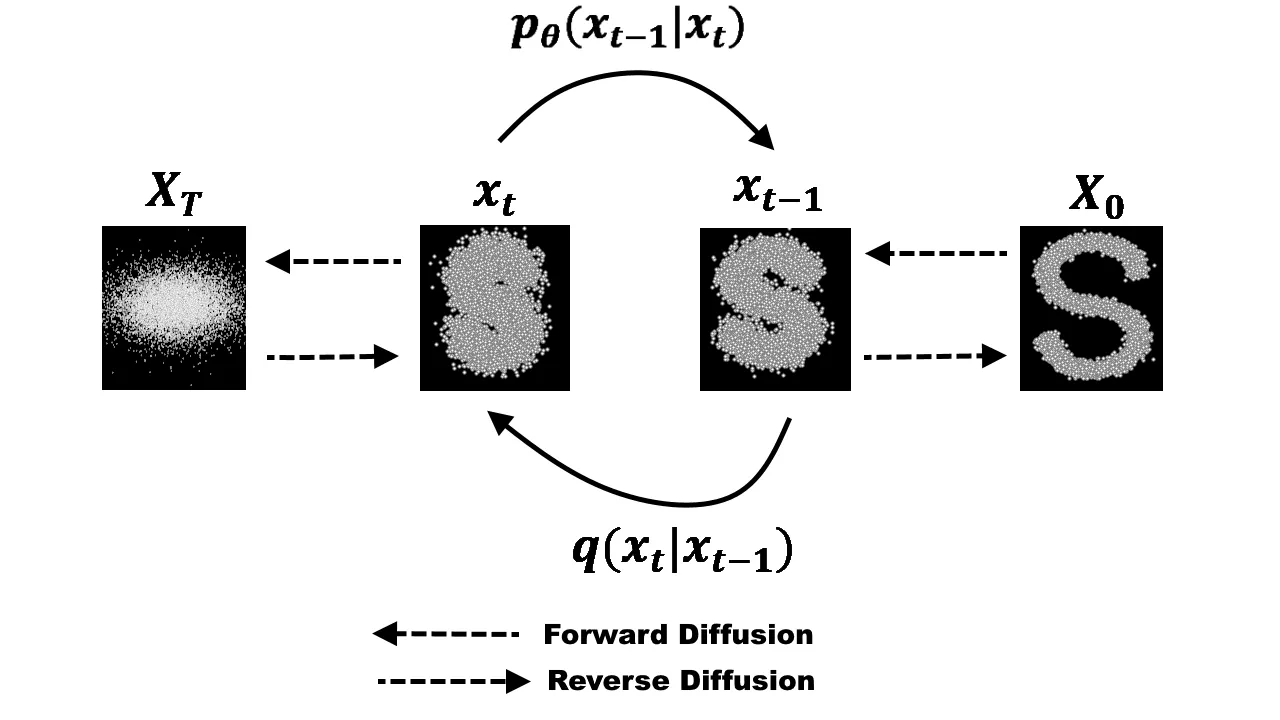
\includegraphics[scale = 0.2]{ThuThesis_ Tsinghua University Thesis LaTeX Template/Picture/Diffusion.png}
        %     \caption{扩散模型图例}
        %     \label{Diffusion}
        % \end{figure}
选取足够大的$T$值与合适的递减序列$\{\beta_t\}_{t\geq 1}$, 条件概率分布$q(x_{T}|x_0)$可以足够接近标准高斯分布。
整个概率系统可以通过变分推断来进行端到端的训练,从而优化参数。
在该模型下,同样采用极大似然估计的方式来进行参数优化,此处采用最大化对数似然函数的相反数的上界来进行优化,即
\begin{equation}
    \mathbb{E}\left[-\log p_\theta\left(\mathbf{x}_0\right)\right] \leq \mathbb{E}_q\left[-\log \frac{p_\theta\left(\mathbf{x}_{0: T}\right)}{q\left(\mathbf{x}_{1: T} \mid \mathbf{x}_0\right)}\right]=\mathbb{E}_q\left[-\log p\left(\mathbf{x}_T\right)-\sum_{t \geq 1} \log \frac{p_\theta\left(\mathbf{x}_{t-1} \mid \mathbf{x}_t\right)}{q\left(\mathbf{x}_t \mid \mathbf{x}_{t-1}\right)}\right]=: L
    \label{DDPM objective 1}
\end{equation}
从随机优化方法的角度去考虑,可以将式(\ref{DDPM objective 1})重新写为
\begin{equation}
\mathbb{E}_q[\underbrace{\mathcal{D}_{K L}\left(q\left(x_T \mid x_0\right) \| p\left(x_T\right)\right)}_{L_T}+\sum_{t>1} \underbrace{\mathcal{D}_{K L}\left(q\left(x_{t-1} \mid x_t, x_0\right) \| p_\theta\left(x_{t-1} \mid x_t\right)\right)}_{L_{t-1}}-\underbrace{\log p_\theta\left(x_0 \mid x_1\right)}_{L_0}]
    \end{equation}
以上为DDPM的数学原理,以下将具体讨论DDPM在实际优化过程中的参数设计与模型细节。以上已经将$L$分解成$L_T,L_{t-1},L_0$三大部分,由于后验分布$q$没有任何参数,因此$L_T$可以直接忽略(和$\theta$取值近似无关)。
在\cite{DDPM}中直接假设$\Sigma_{\theta}(x_t,t)=\sigma_t^2 I$,方便简化计算过程(避免矩阵求逆运算操作)。其次,为了表示$\mu_{\theta}(x_t,t)$,由于$p_{\theta}(x_{t-1}|x_t):= \mathcal{N}(x_{t-1};\mu_{\theta}(x_t,t),\sigma_t^2I)$,我们可以将$L_{t-1}$写为
\begin{equation}
    L_{t-1}=\mathbb{E}_q\left[\frac{1}{2 \sigma_t^2}\left\|\tilde{{\mu}}_t\left(\mathbf{x}_t, \mathbf{x}_0\right)-{\mu}_\theta\left(\mathbf{x}_t, t\right)\right\|^2\right]+C
    \label{Lt representation}
\end{equation}
其中$C$为一个和$\theta$无关的常数,在优化过程中可以被忽略。利用式(\ref{posterior of xt})可以进一步简化式(\ref{Lt representation}) 将$x_t$表示为$\mathbf{x}_t\left(\mathbf{x}_0, {\epsilon}\right)=\sqrt{\bar{\alpha}_t} \mathbf{x}_0+\sqrt{1-\bar{\alpha}_t} {\epsilon} \text { for } {\epsilon} \sim \mathcal{N}(\mathbf{0}, \mathbf{I}) $, 以及利用式(\ref{posterior xt 2})可以得到
\begin{align}
    L_{t-1}-C&=\mathbb{E}_{\mathbf{x}_0, {\epsilon}}\left[\frac{1}{2 \sigma_t^2}\left\|\tilde{{\mu}}_t\left(\mathbf{x}_t\left(\mathbf{x}_0, {\epsilon}\right), \frac{1}{\sqrt{\bar{\alpha}_t}}\left(\mathbf{x}_t\left(\mathbf{x}_0, {\epsilon}\right)-\sqrt{1-\bar{\alpha}_t} {\epsilon}\right)\right)-{\mu}_\theta\left(\mathbf{x}_t\left(\mathbf{x}_0, {\epsilon}\right), t\right)\right\|^2\right]\\
&=\mathbb{E}_{\mathbf{x}_0, {\epsilon}}\left[\frac{1}{2 \sigma_t^2}\left\|\frac{1}{\sqrt{\alpha_t}}\left(\mathbf{x}_t\left(\mathbf{x}_0, {\epsilon}\right)-\frac{\beta_t}{\sqrt{1-\bar{\alpha}_t}} {\epsilon}\right)-{\mu}_\theta\left(\mathbf{x}_t\left(\mathbf{x}_0, {\epsilon}\right), t\right)\right\|^2\right]
\end{align}
经过\cite{DDPM,score_based_SDE}中的计算化简,\ref{DDPM objective 1}实际上可以化简为
\begin{equation}
    \mathbb{E}_{t\sim \mathcal{U}(0,1),\epsilon\sim \mathcal{N}(0,I)}\left[\|\epsilon - \epsilon^{\theta}(x_t,t)\|^2\right]
\end{equation}
而此时的打分函数满足$s^{\theta}(x_t,t) =- \frac{1}{\sqrt{\Bar{\beta}_t}}\epsilon^{\theta}(x_t,t)$,取 $\mu^{\theta}(x_t,t) = \frac{1}{\sqrt{\Bar{\alpha}_t}}\left(x_t- \sqrt{\Bar{\beta}_t}\epsilon^{\theta}(x_t,t)\right)$。 以上为DDPM主要的实现原理与优化过程。

在当下利用Diffusion Model实现图像去噪,图像修损任务中的研究中,主要采用DDPM模型中的随机微分方程进行向前扩散,以及采用和Langevin dynamic 中进行Score matching的方法进行混合使用提升收敛速率。但是实质并没有充分利用图像加噪和去噪随机变量之间的条件分布,本质上是在实现更高效率的生成式模型进行图像还原。下面进行前向加噪模型的一般形式阐述。

前向加噪模型可以总体以如下形式表达:
\begin{equation}
y=\mathcal{H}\left(x_0\right)+{n}, \quad y, {n} \in \mathbb{R}^n, x \in \mathbb{R}^d,
\label{Forward model}
\end{equation}
其中$x_0$为原始分布,即为初始图像采样样本,$y$为加过噪声处理后的图像,$\mathcal{H}$为加噪算符,而$n$表示随机噪声。首先仅考虑$n$为高斯噪声的情况,即$n\sim \mathcal{N}(0,\sigma^2 I_n)$。即$y$服从条件概率分布,$y\sim \mathcal{N}(\mathcal{H}(x_0)\mid \sigma^2 I_n)$。
进一步简化问题,以及考虑实际应用中的下游任务主要集中于降噪,图像修复,去模糊化处理,超分辨率化以及等情形,在此处可假设$\mathcal{H}(\cdot)$为线性变换(线性变换可以适用于图像平移,旋转,图像部分缺损等实际应用场景),对于较为复杂的加噪模型可以在未来的工作中用泛化能力更强的模型进行去噪处理。      
\begin{definition}[图像去噪]
在加噪模型(\ref{Forward model})下,对于加噪后的图像$y$而言存在非唯一的原像。在已知去噪前图像分布数据集$p(x)$的分布和加噪图像后验分布$p(y\mid x)$的条件下,目标是得到$p(x)$内的一个子分布使得最大化后验分布$p(x\mid y)$,即采样得到原图像分布内最有可能经过加噪处理得到目标加噪图片的图像集合的分布。
\end{definition}

在图像去噪任务中,主要目标可以阐释为,在已知加噪后的图像$y$的情形下,还原得到最契合去噪前原始图像的图像分布$x$,即找到最合适的随机分布$x\sim p(x)$,使得
\begin{equation}
    x^{*} = \arg \max_{x\in \mathcal{X}}\log p( x\mid y),
\end{equation}
其中$\mathcal{X}$为可能的图像分布的取值集合空间,相比于在diffusion model中极大化似然函数$\log(p(x))$,此处相当于变成了条件概率分布意义下的似然函数。若同样设计DDPM中的随机微分方程作为向前扩散模型, 则只需要通过拟合条件概率分布意义下的打分函数Score function $\nabla_{x_t}\log\left(p(x_t\mid y)\right)$。   






对于噪声$n$的分布也可以设置一定的先验假设。如果仅考虑$n$为高斯噪声的情形,则条件似然函数有以下形式:
\begin{equation}
 p\left(y \mid x_0\right)=\frac{1}{\sqrt{(2 \pi)^n \sigma^{2 n}}} \exp \left[-\frac{\left\|y-\mathcal{H}\left(x_0\right)\right\|_2^2}{2 \sigma^2}\right],
 \label{log-likelihood gaussion }
\end{equation}
根据Bayes公式我们有
\begin{equation}
    p_t(x_t\mid y) = \frac{p_t(x_t)}{p_t(y)}\cdot p_t(y\mid x_t),
\end{equation}
用到$\nabla_{x_t}p_t(y)=0$, 因此可以化简得到如下结果
\begin{equation}
\nabla_{x_t} \log p_t\left(x_t \mid y\right)=\nabla_{x_t} \log p_t\left(x_t\right)+\nabla_{x_t} \log p_t\left(y \mid x_t\right).
\label{conditional score function }
\end{equation}
因此在本图像去噪任务中最重要的任务即为如何拟合函数$\log \left(p(y\mid x_t)\right)$。

该问题的困难之处在于,如果重新训练一个新的模型用来逼近该打分函数,计算量上的难度较大,以及会有较大的重构误差(reconstruction error)。因此需要引入新的方法来进行建模。在\cite{song_2}中采用先用$x_t$替代$x_0$再对条件概率分布下的方差进行手动调整的方法逼近打分函数,即
\begin{equation}
    \nabla_{x_t}\log\left(p(y\mid x_t)\right) \approx \nabla_{x_t}\left(-\frac{\|y-Hx_t\|^2}{2\left(\sigma_y^2+\gamma_t^2\right)}\right) = \frac{H^{\top}(Hx_t-y)}{\sigma_y^2+\gamma_t^2},
    \label{approx MRI}
\end{equation}
该方法的优点在于不需要重新训练模型,只需要(\ref{approx MRI})中的具有解析形式的函数去逼近现有的条件概率分布下的Score function (\ref{conditional score function }),而$\nabla_{x_t}\log\left(p(x_t)\right)$可以直接使用预训练的模型进行使用,因此该方法较为简便在计算效率上具有高效性。缺点在于超参数$\{\gamma_t\}_{t\geq 0}$需要进行人为选择,以及直接使用$x_t$替代$x_0$, 对于真实的概率分布的逼近效果没有理论上的保证。



我们的总体思路如下,根据原始图像$x_0$与给定的随机微分方程\ref{diffusion equation SDE 1}得到随机过程$\{x_t\}_{t\in [0,T]}$, 使得$x_T$为分布可知的随机变量。 再利用极大似然估计的方法极大化$\log\left(p_{\theta}(x_0\mid y)\right)$ 从而得到相应的逆向过程。核心即为,在极大化条件似然函数的情况下,得到相应新的打分函数$\nabla_{x_t}\log(q_t(x_t\mid y))$。从而可以通过逆向随机微分方程得到相应的随机变量分布进行采样。

借鉴\cite{DDPM}中的原理,可以选取形式较为简单的随机微分方程形式来实现扩散模型。例如在VE SDE(Variance Exploding SDE)下,选取$f(x,t)=0$以及$g(t) = \sqrt{\frac{d}{dt}\sigma^2(t)}$,则相邻两个随机变量的采样过程可以表示为
\begin{equation}
    x_{(i+1)} = x_{i}+\sqrt{\sigma_i^2-\sigma_{i-1}^2}z_{i-1}, z_{i-1}\sim \mathcal{N}(0,I)
\end{equation}


在该条件下, 前向传播条件密度函数 
\begin{equation}
  q\left(x_t \mid x_{t-1}\right)=\mathcal{N}\left(x_{t-1},\left(\sigma_t^2-\sigma_{t-1}^2\right) I\right), q\left(x_t \mid x_0\right)=\mathcal{N}\left(x_0, \sigma_t^2 I\right),  
\end{equation}
, 以及我们还有
\begin{equation}
    q\left(x_{t-1} \mid x_t, x_0\right)=\mathcal{N}\left(\frac{\sigma_{t-1}^2}{\sigma_t^2} x_t+\left(1-\frac{\sigma_{t-1}^2}{\sigma_t^2}\right) x_0, \frac{\sigma_{t-1}^2}{\sigma_t^2}\left(\sigma_t^2-\sigma_{t-1}^2\right) l\right) .
\end{equation}
在进行非去噪任务,单纯进行非条件生成的时候,逆向生成可以采用如下方式:
\begin{equation}
    x_{t-1}=\frac{\sigma_{t-1}^2}{\sigma_t^2} x_t+\left(1-\frac{\sigma_{t-1}^2}{\sigma_t^2}\right) \hat{x}_0\left(x_t\right)+\frac{\sigma_{t-1}}{\sigma_t} \sqrt{\sigma_t^2-\sigma_{t-1}^2} \epsilon, \quad \epsilon \sim \mathcal{N}(0, I)
\end{equation}
其中我们有$\hat{x}_0\left(x_t\right)=\mathbb{E}\left[x_0 \mid x_t\right]=x_t+\sigma_t^2 \nabla_{x_t} \log p_t\left(x_t\right)$, 则我们可以将如上生成公式写成如下形式
\begin{equation}
    x_{t-1}=x_t+\left(\sigma_t^2-\sigma_{t-1}^2\right) s_\theta\left(x_t, \sigma_t\right)+\frac{\sigma_{t-1}}{\sigma_t} \sqrt{\sigma_t^2-\sigma_{t-1}^2} \epsilon=: f\left(x_t ; t\right), \quad \epsilon \sim \mathcal{N}(0, I).
    \label{reverse sampling}
\end{equation}
在\cite{song_2,DDPM}中主要运用学习到的Score function来进行逆向采样得到对目标分布的逼近。在条件生成任务中,类比无条件生成中的情形,可以利用相似的原理对条件概率分布下的Score function来进行逆向分布。在\cite{Inverse}中通过对$p(x_0\mid x_t)$的逼近来得到对$p(y\mid x_t)$的逼近,从而可以实现逆向采样。
同样,在\cite{Inverse}中考察了在选取VP-SDE(Variance Preserving SDE)下的采样过程,主要如下:      

1. 先通过$x_t$得到$\hat{x}_0$,即
\begin{equation}
    \hat{{x}}_0 \leftarrow \frac{1}{\sqrt{\bar{\alpha}_t}}\left({x}_t+\left(1-\bar{\alpha}_t\right) \hat{{s}}(x_t,t)\right).
\end{equation}
        
        2.再生成白噪声用于后续生成,即生成噪声$z$,
\begin{equation}
    {z} \sim \mathcal{N}(\mathbf{0}, {I}) 
\end{equation}
      
      
      3. 最后再根据DDPM下的采样方法进行条件采样
\begin{equation}
     {x}_{i-1}^{\prime} \leftarrow \frac{\sqrt{\alpha_i}\left(1-\bar{\alpha}_{i-1}\right)}{1-\bar{\alpha}_i} {x}_i+\frac{\sqrt{\bar{\alpha}_{i-1}} \beta_i}{1-\bar{\alpha}_i} \hat{{x}}_0+\tilde{\sigma}_i {z}
\end{equation}


以及在DDPM设置的模型下,有如下两个结论可以帮助逼近$p(y\mid x_t)$:

\begin{proposition}
\label{prop 1}
     在使用DDPM条件下的随机微分方程进行向前采样的扩散模型下, $p\left(x_0 \mid x_t\right)$ 有唯一的后验概率分布下的数学期望
$$
\hat{x}_0:=\mathbb{E}\left[x_0 \mid x_t\right]=\frac{1}{\sqrt{\bar{\alpha}(t)}}\left(x_t+(1-\bar{\alpha}(t)) \nabla_{x_t} \log p_t\left(x_t\right)\right)
$$
\end{proposition}
\begin{theorem}
\label{thm 1}
对于给定的线性加噪模型(\ref{Forward model}) 满足噪声分布${n} \sim \mathcal{N}\left(0, \sigma^2 {I}\right)$,我们有如下渐进分析结果
\begin{equation}
  p\left(y \mid x_t\right) \approx p\left(y \mid \hat{x}_0\right),
  \label{Thm 1 eq 1}
\end{equation}

其中逼近误差可以利用詹森误差\footnote{詹森误差定义:$\mathcal{J}(f,x\sim p(x)) = \mathbb{E}[f(x)]-f(\mathbb{E}[x])$, 其中数学期望是在服从$p(x)$概率分布意义下的数学期望}来表示,其上界为
\begin{equation}
\mathcal{J} \leq \frac{d}{\sqrt{2 \pi \sigma^2}} e^{-1 / 2 \sigma^2}\left\|\nabla_{x} \mathcal{H}(x)\right\| m_1,
    \label{upper bound thm 1}
\end{equation}
其中我们还有
\begin{equation}
    \left\|\nabla_{x} \mathcal{H}(x)\right\|:=\max _{x}\left\|\nabla_{x} \mathcal{H}(x)\right\|,
\end{equation}
以及
\begin{equation}
m_1:=\int_{\mathbb{R}^d}\left\|x_0-\hat{x}_0\right\| p\left(x_0 \mid x_t\right) d x_0  
\end{equation}
\end{theorem}
根据\ref{prop 1}和\ref{thm 1}的结论,可以通过$p(y\mid \hat{x}_0(x_t))$来得到对与$p(y\mid x_t)$
的逼近。在\cite{Inverse}中,在每一步逆向采样中,主要分为两步:   

(i)首先根据在无条件生成情况下,根据Diffusion Model的结构,通过(\ref{reverse sampling})进行一步逆向采样,通过$x_i$得到$x_{i-1}^{\prime}$。    

(ii)再通过估计$\nabla_{x_t}\log(p(y\mid x_t))$,通过$x_{i-1}^{\prime}$得到$x_{i-1}$,具体更新形式为
\begin{equation}
    x_{i-1} \leftarrow x_{i-1}^{\prime}-\zeta_i \nabla_{x_i}\left\|y-\mathcal{H}\left(\hat{x}_0\right)\right\|_2^2, \label{update 2 DPS}
\end{equation}
其中$\zeta_i$为预先设定的步长。

在\cite{Inverse}提出的条件生成算法中,只需要前向加噪满足自动微分条件,即可以得到$\nabla_x\mathcal{H}(x)$,则可以对无论线性或者非线性加噪模型均进行图像修复任务。相比于传统图像修复任务中对于$\mathcal{H}$均假设为线性有了较大的创新性和适用范围,以及不需要获取过多对于$\mathcal{H}$的信息。     

但是该算法的局限性在于      


1. 需要手动设置步长$\{\zeta_i\}_{i\geq 1}$,对于不同的数据集选用的相应取值需要进行调整。 而步长实际对应为后验概率分布下的方差,即$\operatorname{Var}\left[y\mid x_t\right]$,在\cite{song2023pseudoinverse,Inverse}中均采用选取对其估计值的方法人工指定步长,会带来一定的误差。   


2. 使用DDPM模型作为基准扩散模型进行反向采样,但是采样过程中需要对整条链进行生成。若采用DDIM等模型进行替代,结合\cite{DDIM},则可以在不需要生成整条链的情况下进行图像生成,相比于原先的情形有了较大的效率上的提升。   

3. 以及噪声预测神经网络结构中只使用了在\cite{Unet}中提出的Unet神经网络结构,可以结合在\cite{DDIM,VAE_diffusion}中所提出结合transformer模型所利用的attention机制,进一步提升模型性能。     

4.在\cite{Inverse}中所提出的方法目前仅仅在FFHQ10数据集上得到验证,在如Imagenet等数据集上的具体效果有待后续进行测试。    

根据以上局限性,后续可以进行如下工作
\begin{itemize}
    \item 构造DDIM模型下的条件生成任务,结合\cite{song2023pseudoinverse}中提出的Pseudoinverse 算法,在\cite{Inverse}基础上进一步增强生成效率.
    \item  尝试改善在\cite{Inverse}中较为随意的$\{\zeta_i\}_{i\geq 1}$方式,得到更加精确的后验方差估计,可结合在\cite{Analytic_DPM}中对model-free 假设下最佳后验估计的结果。
    \item 尝试在不同数据集下使用DPS算法的生成效果,目前的DPS算法仅在FFHQ10数据集下进行实现。
    \item \textbf{在时间允许的情况下},对原先的Unet结构加入transformer结构增强模型泛化能力。
    
\end{itemize}

\chapter{实验分析}
在本章中主要阐述图像去噪生成算法的具体实现流程,工程架构和实验结果分析。 首先,




以下对具体数据集进行实验分析
\begin{table}[H]
    \centering
    \begin{tabular}{|c|c|c|c|c|}
\hline \multirow[b]{2}{*}{ Method } & \multicolumn{2}{|c|}{ Inpaint (random)} & \multicolumn{2}{|c|}{ Inpaint (box) } \\
\hline & PSNR $\uparrow$ & $\operatorname{SSIM} \uparrow$ & PSNR $\uparrow$ & $\operatorname{SSIM} \uparrow$ \\
\hline \text{本文算法} & $\underline{23.87}$ & $\underline{0.781}$ & 18.90 & $\underline{0.794}$ \\
\hline DPS\cite{Inverse}  & $\underline{23.87}$ & $\underline{0.781}$ & 18.90 & $\underline{0.794}$ \\
\hline DDRM \cite{ddrm} & 24.96 & 0.790 & $\underline{18.66}$ & 0.814 \\
\hline MCG\cite{MCG}  & 13.39 & 0.227 & 17.36 & 0.633 \\
\hline PnP-ADMM\cite{PnP}  & 23.75 & 0.761 & 12.70 & 0.657 \\
\hline \begin{tabular}{l} 
Score-SDE \cite{score_based_SDE} \\
\end{tabular} & 12.25 & 0.256 & 16.48 & 0.612 \\
\hline ADMM-TV & 22.17 & 0.679 & 17.96 & 0.785 \\
\hline
\end{tabular}
\end{table}






% 其他部分
\backmatter

% 参考文献
\bibliography{ref/refs}  % 参考文献使用 BibTeX 编译
% \printbibliography       % 参考文献使用 BibLaTeX 编译

% 附录
% 本科生需要将附录放到声明之后,个人简历之前
\appendix
% !TeX root = ../thuthesis-example.tex

\begin{survey}
\label{cha:survey}

\title{Literature Review}
\maketitle


% \tableofcontents

The field of image restoration has witnessed a paradigm shift with the advent of deep learning technologies. Among these, diffusion models have emerged as particularly potent, owing to their ability to reconstruct high-quality images from corrupted inputs. This review delves into the evolution and contributions of diffusion models, especially focusing on Score-Based Stochastic Differential Equations \cite{score_based_SDE}, Denoising Diffusion Probabilistic Models \cite{DDPM}, and Denoising Diffusion Implicit Models \cite{DDIM}, while also discussing the role of Variational Autoencoders \cite{VAE_diffusion} and the integration of manifold constraint learning \cite{MCG}.  VAEs, as introduced by \cite{vae_model}, marked a significant milestone in image restoration, providing a framework for modeling complex image distributions. Despite their contributions, the quest for models that better capture high-dimensional data distributions led to the exploration of diffusion models, which offer a novel approach to image restoration.       

Diffusion models, particularly DDPM, introduced by \cite{DDPM}, have redefined image restoration strategies. These models employ a reverse diffusion process to generate data from noise, demonstrating unparalleled performance in handling complex image degradations.    


The incorporation of Score-Based SDEs into diffusion models, as explored by \cite{score_based_SDE,song_2}, has further enhanced the field. These models use the data distribution's score-based gradient for a more refined denoising process, leading to superior restoration quality.    

DDIM, a notable advancement over DDPM, was introduced by \cite{DDIM} to improve efficiency in the denoising process. This model significantly accelerates image restoration without compromising output quality, highlighting its potential for real-time applications.   

Manifold constraint learning has been pivotal in ensuring that restored images adhere to natural image characteristics. The integration of this concept with diffusion models, especially in works like \cite{Inverse,PnP,MCG}, demonstrates significant improvements in photorealism and structural coherence.      


Recent literature has expanded the scope of diffusion models in image restoration. The DDRM framework, as discussed by \cite{ddrm}, and the Pseudo Inverse Algorithm \cite{red_diff} offer novel approaches to tackling image restoration tasks, emphasizing the versatility and depth of diffusion-based methodologies. Furthermore, the emergence of consistency models \cite{Consistency} and Stable Diffusion  \cite{vae_model} highlight the ongoing innovation within the domain, promising even more sophisticated solutions to image restoration challenges.       


The exploration of diffusion models in image restoration has ushered in a new era of possibilities, with DDPM, DDIM, and the integration of Score-Based SDEs representing significant advancements. The addition of manifold constraint learning and the exploration of new models like DDRM and the Pseudo Inverse Algorithm further enrich the field. As research continues to evolve, the foundational works and recent innovations collectively point towards a future where image restoration achieves unprecedented levels of accuracy and realism.



\bibliographystyle{unsrtnat}
\bibliography{ref/refs}

\end{survey}
       % 本科生:外文资料的调研阅读报告
% % !TeX root = ../thuthesis-example.tex

\begin{translation}
\label{cha:translation}

\title{书面翻译题目}
\maketitle

\tableofcontents


本科生的外文资料书面翻译。


\section{图表示例}

\subsection{图}

附录中的图片示例(图~\ref{fig:appendix-translation-figure})。

\begin{figure}
  \centering
  \includegraphics[width=0.6\linewidth]{example-image-a.pdf}
  \caption{附录中的图片示例}
  \label{fig:appendix-translation-figure}
\end{figure}


\subsection{表格}

附录中的表格示例(表~\ref{tab:appendix-translation-table})。

\begin{table}
  \centering
  \caption{附录中的表格示例}
  \begin{tabular}{ll}
    \toprule
    文件名          & 描述                         \\
    \midrule
    thuthesis.dtx   & 模板的源文件,包括文档和注释 \\
    thuthesis.cls   & 模板文件                     \\
    thuthesis-*.bst & BibTeX 参考文献表样式文件    \\
    thuthesis-*.bbx & BibLaTeX 参考文献表样式文件  \\
    thuthesis-*.cbx & BibLaTeX 引用样式文件        \\
    \bottomrule
  \end{tabular}
  \label{tab:appendix-translation-table}
\end{table}


\section{数学公式}

附录中的数学公式示例(公式\eqref{eq:appendix-translation-equation})。
\begin{equation}
  \frac{1}{2 \uppi \symup{i}} \int_\gamma f = \sum_{k=1}^m n(\gamma; a_k) \mathscr{R}(f; a_k)
  \label{eq:appendix-translation-equation}
\end{equation}


\section{文献引用}

文献引用示例\cite{abrahams99tex}。


\appendix

\section{附录}

附录的内容。


% 书面翻译的参考文献
\bibliographystyle{unsrtnat}
\bibliography{ref/appendix}

% 书面翻译对应的原文索引
\begin{translation-index}
  \nocite{salomon1995advanced}
  \bibliographystyle{unsrtnat}
  \bibliography{ref/appendix}
\end{translation-index}

\end{translation}
  % 本科生:外文资料的书面翻译
% !TeX root = ../thuthesis-example.tex

\chapter{补充内容}
\label{appendix}
\section{插图}
以下为在FFHQ数据集上测试的结果展示
\begin{figure}[H]
  \centering
  \begin{minipage}[b]{0.3\linewidth}
\includegraphics[width=\linewidth]{Picture/input/00004.png}
    \caption{加噪图像4}
    \label{noised image }
  \end{minipage}
  \hspace{0.1cm} % Space between images
   \begin{minipage}[b]{0.3\linewidth}
    \includegraphics[width=\linewidth]{Picture/label/00004.png}
    \caption{原始图像4}
    \label{original image }
  \end{minipage}
\hspace{0.1cm}
  \begin{minipage}[b]{0.3\linewidth}
    \includegraphics[width=\linewidth]{Picture/recon/00004.png}
    \caption{还原图像4}
    \label{inpainted image}
  \end{minipage}
\end{figure}



\begin{figure}[H]
  \centering
  \begin{minipage}[b]{0.3\linewidth}

\includegraphics[width=\linewidth]{Picture/input/00005.png}
    \caption{加噪图像5}
    \label{noised image }
  \end{minipage}
  \hspace{0.1cm} % Space between images
   \begin{minipage}[b]{0.3\linewidth}
    
\includegraphics[width=\linewidth]{Picture/label/00005.png}
    \caption{原始图像5}
    \label{original image }
  \end{minipage}
\hspace{0.1cm}
  \begin{minipage}[b]{0.3\linewidth}
    
\includegraphics[width=\linewidth]{Picture/recon/00005.png}
    \caption{还原图像5}
    \label{inpainted image}
  \end{minipage}
\end{figure}

\begin{figure}[H]
  \centering
  \begin{minipage}[b]{0.3\linewidth}
\includegraphics[width=\linewidth]{Picture/input/00006.png}
    \caption{加噪图像6}
    \label{noised image }
  \end{minipage}
  \hspace{0.1cm} % Space between images
   \begin{minipage}[b]{0.3\linewidth}
    \includegraphics[width=\linewidth]{Picture/label/00006.png}
    \caption{原始图像6}
    \label{original image }
  \end{minipage}
\hspace{0.1cm}
  \begin{minipage}[b]{0.3\linewidth}
    \includegraphics[width=\linewidth]{Picture/recon/00006.png}
    \caption{还原图像6}
    \label{inpainted image}
  \end{minipage}
\end{figure}


\section{实验说明}
本项目为开源项目,可以直接从github上获取本项目代码,在终端输入如下命令行。1. 拷贝项目
\label{experiment instructions}
\begin{lstlisting}[language=bash]
git clone git@github.com:JamesJunyuGuo/Graduation_Project.git
cd Graduation_Project/
\end{lstlisting}
2. 下载预训练集。 参考github仓库\href{https://github.com/openai/guided-diffusion.git}{https://github.com/openai/guided-diffusion.git}可以点击进入网页下载对应的预训练集。在主文件夹中新建一个新文件夹 models/ 并将下载的预训练集放到里面。
\begin{lstlisting}[language=bash]
mkdir models
mv {DOWNLOAD_DIR}/ffqh_10m.pt ./models/
mv {DOWNLOAD_DIR}/lsun_bedroom.pt ./models/
\end{lstlisting}
3. 本地环境配置
\begin{lstlisting}[language=bash]
conda create --name DM python=3.8

conda activate DM

pip install -r requirements.txt

pip install torch==2.2.2
\end{lstlisting}
4. 训练过程   
执行训练只需要在本地命令行输入如下代码
\begin{lstlisting}[language=bash]
python3 sample_test.py \
--model_config=configs/LSUN_config.yaml \
--diffusion_config=configs/diffusion_config.yaml \
--task_config=inpainting_config.yaml;
\end{lstlisting}
其中可以根据具体的下游任务类型修改yaml文件中的具体配置,例如在任务设置参数中可以修改root以及name更改读取数据集位置以为选取不同的下游任务进行训练,文件配置内容如下可见。
\begin{lstlisting}[language=bash]
conditioning:
    method: ddim 
    params:
        scale: 1.0

data:
    name: LSUN
    root: ./data/samples/

measurement:
    operator: 
        name: inpainting # check candidates in guided_diffusion/measurements.py

noise:
    name:  gaussian 
    sigma:  0.05 
\end{lstlisting}








% 致谢
% !TeX root = ../thuthesis-example.tex

\begin{acknowledgements}
  衷心感谢导师×××教授和物理系××副教授对本人的精心指导。他们的言传身教将使我终生受益。

  在美国麻省理工学院化学系进行九个月的合作研究期间,承蒙 Robert Field 教授热心指导与帮助,不胜感激。

  感谢×××××实验室主任×××教授,以及实验室全体老师和同窗们学的热情帮助和支持!

  本课题承蒙国家自然科学基金资助,特此致谢。
\end{acknowledgements}


% 声明
\statement
% 将签字扫描后的声明文件 scan-statement.pdf 替换原始页面
% \statement[file=scan-statement.pdf]
% 本科生编译生成的声明页默认不加页脚,插入扫描版时再补上;
% 研究生编译生成时有页眉页脚,插入扫描版时不再重复。
% 也可以手动控制是否加页眉页脚
% \statement[page-style=empty]
% \statement[file=scan-statement.pdf, page-style=plain]

% 个人简历、在学期间完成的相关学术成果
% 本科生可以附个人简历,也可以不附个人简历
% \input{data/resume}

% 指导教师/指导小组评语
% 本科生不需要
% !TeX root = ../thuthesis-example.tex

\begin{comments}
% \begin{comments}[name = {指导小组评语}]
% \begin{comments}[name = {Comments from Thesis Supervisor}]
% \begin{comments}[name = {Comments from Thesis Supervision Committee}]

  论文提出了……

\end{comments}


% 答辩委员会决议书
% 本科生不需要
% !TeX root = ../thuthesis-example.tex

\begin{resolution}

  论文提出了……

  论文取得的主要创新性成果包括:

  1. ……

  2. ……

  3. ……

  论文工作表明作者在×××××具有×××××知识,具有××××能力,论文××××,答辩××××。

  答辩委员会表决,(×票/一致)同意通过论文答辩,并建议授予×××(姓名)×××(门类)学博士/硕士学位。

\end{resolution}


% 本科生的综合论文训练记录表(扫描版)
% \record{file=scan-record.pdf}

\end{document}
